\documentclass[oneside]{book}
\usepackage[pdftex]{graphicx}
\usepackage{setspace,amssymb,amsmath,epstopdf,natbib,amsthm}
\usepackage[usenames,dvipsnames]{color}
\usepackage{pifont}
\usepackage{xr}
\usepackage{listings}
\usepackage[hidelinks]{hyperref}  % Likes to be the last class loaded
\hypersetup{bookmarksdepth=2}
\externaldocument[A-]{NeuralNetworksCogsci}

\def\ie{{\it i.e. }}
\def\eg{{\it e.g. }}
\newcommand{\code}{\texttt}

%
% Use this command to indicate glossary entries. Be sure some entry of the same name
% exists in Glossary.txt
%
\def\glossary{\textbf}

%
% extref is a reference to a label that may or may not exist in the current subdocument. 
% If it does, a regular reference is produced. If it is not found in the current subdocument,
% a reference to the label in the master document is given, and a * is added to indicate this.
% Note that this only works if the master document has been compiled
%
% Example (cf. Chapter \extef{ch_intro}) compiles to:
% (cf. Chapter 1) 	If the chapter is in the subdocument
% (cf. Chapter 1*) 	If the chapter is not in the subdocument
%
\makeatletter
\newcommand{\extref}[1]{\@ifundefined{r@#1}{\ref{A-#1}$^*$}{\ref{#1}}}
\makeatother

%
% Use this command to designate chapter authors. An optional second command indicates 
% their relative contribution to the chapter. 
%
% Example: \chapterauthor{Scott Hotton, Chelsea Gordon, Jeff Yoshimi}{.5,.3,2}
%
% If the second argument is not used, it is assumed all chapter authors contributed equally. 
%
\makeatletter
\newcommand{\chapterauthor}[2]{%
  {\parindent0pt\vspace*{-25pt}%
  \linespread{1.1}\large\scshape#1%
  \par\nobreak\vspace*{35pt}}
  \@afterheading%
}
\makeatother

% Renaming ``List of Figures'' to  ``Figure Attributions''
\renewcommand*\listfigurename{Figure Attributions}

\setlength{\textwidth=6.5in}
\setlength{\textheight=9.0in}
\hoffset=-0.80in
\voffset=-1.00in

\begin{document}

%\tableofcontents

% Choose which chapters to include here by uncommenting
\chapter{New Material for Linear Algebra}
\chapterauthor{Jeff Yoshimi}

% TODO: Pictures for source-target representations

\subsection{The scalar and vector tracks}

% Compare https://youtu.be/Smav86u60FM?t=390 (from neurons to tokens, from weighted combinations of scalars to weighted combinations of vectors)

%To get to the next belt level, you have to deal with this kind of thing, and so train your brain to deal with it.

The book  can be thought of as involving two tracks: a `scalar' and a `vectorized' track. In the scalar track, we think of all operations from the standpoint of individual neurons and their values. We index weights using a source-target structure. In Simbrain, the focus is mostly on separately presented nodes. We use vectors and matrices to understand many ideas conceptually, but we do not make heavy use of matrix products or matrix algebra. This is much more accessible to beginning students, and is sufficient to teach an entire class. Indeed, this has been the way the book was structured and is the main way Simbrain 3.0 works. This supports the main thrust of the book and Simbrain, making neural networks easy enough to use without any math background at all (there is math to learn, but it is self contained). 
% Source target entails a different representation of matrices

However, this is not how things are done by most professionals working on neural networks in industry, and most academics as well (ch 1 taxonomy). For any serious work, we must move to the vectorized approach. Everything becomes more concise, and runs more efficiently on high performance performance computers. This requires a change in thinking, a way of seeing and thinking about these problems in terms of matrices, vectors, and tensors, often seeing datasets and batches in new ways, almost as tubes of information that get transformed. The focus here is on vectors, matrices, and higher rank tensors, and on applying linear algebra methods directly to these structures. The weights are now indexed using a target-source scheme. The basic objects are mostly matrices, and matrix products--especially multiplications of matrices by column vectors--are the basic operations. In Simbrain 4.0 we have been and are making efforts to make this mode of thinking more intuitive. As of now, there is very little in this format in the book, but we are in the process of adding chapters and sections that present that point of view. Ultimately the hope is to have enough material that a more advanced course could be done entirely from that point of view.

One downside of this is that the indexing changes depending on what you read, but we hope this downside can be an upside. The main book allows a non-math approach, but those going to the target-source point of view must also develop an ability to switch between representations, to see it both ways, which is more complex cognitively but in a way that suits the more advanced mind sets. Many problems are like that, allowing for multiple representations.

% Define shape of matrix
% Transposes.  Also address in line vectors and whether they need the transpose. There's this weird situation. In simbrain and in general, the default is columns.   But in a book, the default is row.  So to show column we do transose operator. But if bold face alone, it is colulmn

\subsection{Graphical conventions}

To think in terms of vectors, we need to bridge between conventional linear algebra notation, and conventional neural network representations, as in Simbrain.  We need a template for mentally moving back and forth between these ways of thinking.  

The first thing to do is get clear on the shape of the matrix. Remember, we are using an ``output-input'' representation.  It feels backwards but it's how it's done.  So, in figure \ref{linalgToSimbrain}, start on the right with Simbrain.  Count the number of outputs, then the number of inputs. Then we have an output-input matrix.  So $3$, $2$, and a $3 \times 2$ matrix.

\begin{figure}[h]
\centering
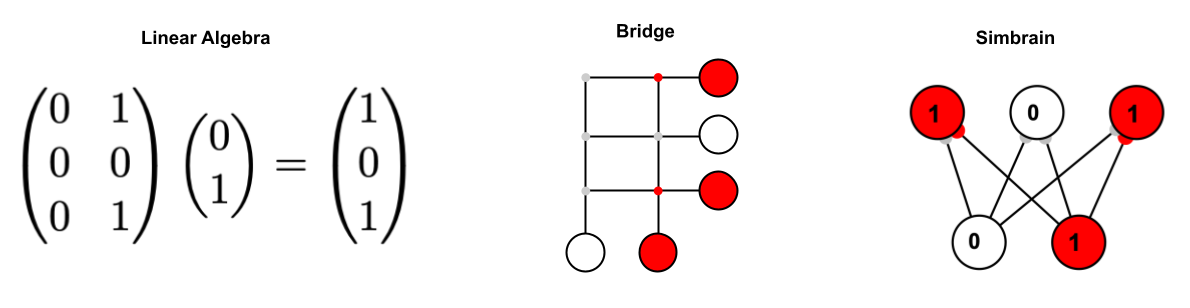
\includegraphics[width=0.75\textwidth]{images/LinalgToSimbrainReps.png}
\caption[Jeff Yoshimi.]{A set of images to help link standard visual representations in linear algebra (left) with standard visual representations of neural networks (right), via the intermediate representation in the middle. }
\label{linalgToSimbrain}
\end{figure}

Figure \ref{linalgToSimbrain} is an effort to bridge this gap. On the left is a standard matrix product, $\mathbf{W} \mathbf{x} = \mathbf{y}$.  This is how forward propagation of an input vector through a weight matrix is usually understood. The weight matrix is $\mathbf{W}$, the input is $\mathbf{x}$, and the output is $\mathbf{y}$. We think of the matrix as operating on the column vector to produce a new column vector.   

% need a transpose section
Here is how I suggest you think about this to connect it up to intuitions about neural networks.  Think of the column vector $\mathbf{x}$ as being rotated 90 degrees or transposed to become a row vector (imagine grabbing the vector by the $1$ and pulling it up and to the right). Now mentally take this row and move it to the bottom of the weight matrix, as in the middle panel of  \ref{linalgToSimbrain}. The weight matrix and the output vector stay in the same orientation.  The fan-out weight vectors from the input are shown as vertical lines, and the fan-in weight vectors to the output are shown as horizontal lines. Now we can easily ``follow'' the activations upwards as activity is propagated. 
% The bridge is pretty close to the new simbrain rep. Show that?
% Note there are other reps too, like the points in a space rep.

I like to think of the input vector as being dotted with each fan-in weight vector on the outputs to produce the entries of the output vector.

To go from the bridge to the standard Simbrain representation in the right panel we now leave the inputs in place, and imagine the outputs being rotated 90 degrees and moved to the top, and imagine the weights kind of following along. Hopefully you can just see it. 

In Simbrain 4.0, we have designed the representation of activation vectors and weight matrices to follow the ``bridge'' concept above as closely as possible.  See figure \ref{simbrain4_ff23}.

\begin{figure}[h]
\centering
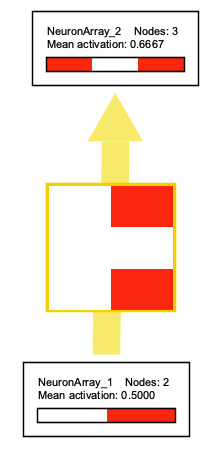
\includegraphics[width=0.15\textwidth]{images/simbrain4_ff_2_3.png}
\caption[Jeff Yoshimi.]{Graphical conventions for activation vectors and weight matrices in Simbrain 4. }
\label{simbrain4_ff23}
\end{figure}
%
%Also just a thought on how to think about the weight matrices. Their shape is target-source, or output-input. So if we have a 3-5-2-1 network in terms of node layers, we have three weight matrices. Their shapes are:
%
%5x3
%2x5
%1x2
%
%So you would pass a list of the form [5x3, 2x5, 1x2] to your function. Remember, weight matrices on the left are multiplied by input and activations vectors on the right.I find this pretty counter-intuitive and takes me a lot of practice to think in this “output-input” way.  I want to read left-to-right input-to-output but the standard conventions with matrix product reverse this...


\chapter{New Material on Unsupervised Learning}
\chapterauthor{Jeff Yoshimi}

\section{Vectorized Hebb Rule}

We've seen how the Hebb rule works for scalar values. Nice and easy: if they fire together, wire together; source times target activations. The situation is the same when we vectorize the rule, but now we have activation vectors $\mathbf{a}_{\text{in}}$ and $\mathbf{a}_{\text{out}}$, and we have to find a vector operations that ``lines up'' the right components of the two vectors so that we strengthen the right ones.  Here is a preview: multiply the output activation column vector times the input row vector (the input transposed, since we assume columns to start), and out pops what we're looking for. 

So, as usual in the vector world, things end up feeling kind of backwards, we multiply output times input rather than the other way around, and there is this mysterious transpose thrown in.  But if we go back to the ``bridge'' panel of the figure above, it ends up making sense. Figure \ref{vectorizedHebb} shows the idea. I like to start in the center panel, and then (to link to the linear algebra) think of the mentally moving the output vector to the left and moving the input vector to the top. Then we have a kind of outer product representation, and all the products kind of line up in the right way. 

\begin{figure}[h]
\centering
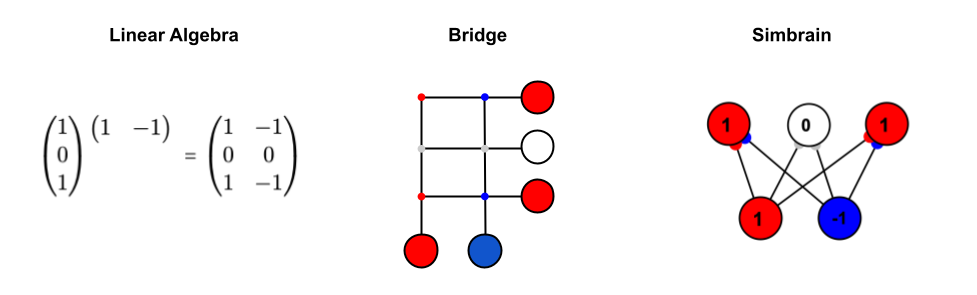
\includegraphics[width=0.9\textwidth]{images/vectorizedHebb.png}
\caption[Jeff Yoshimi.]{Using our visual conventions to conceptualized the vectorized Hebb rule,}
\label{vectorizedHebb}
\end{figure}

As a slogan: output column times input row gives you a weight matrix.

As a sanity check in the example, check the shapes. We have a $3 \times 1$ output vector times a $1 \times 2$ row vectors, which gives us a weight matrix (or weight matrix delta) in the correct shape: $3 \times 2$. This is sometimes called an outer product. So the vectorized Hebb rule is: 

\begin{eqnarray}
\label{vectorHebb}
\Delta \mathbf{W}  = \epsilon \mathbf{a}_{\text{out}} \mathbf{a}_{\text{in}} ^T
\end{eqnarray}
Remember, by default all vectors in bold face are column vectors. We are taking an $n_{out} \times 1$ column vector of output activations and matrix multiplying by a $1 \times n_{in}$ row vector input activations, to produce an $n_{out} \times n_{in}$ matrix in the same shape as the weight matrix.

Suppose we have an input vector $\mathbf{x} = (-1, 1)$, and an output vector $\mathbf{y} = (1,0,1)$ and all the weights are zero, and our learning rate is 1.
\begin{equation*}
\epsilon = 1 \; \; \; \; \\
\mathbf{a}_{\text{in}} = \begin{bmatrix} -1 \\ 1 \end{bmatrix} \\ 
\; \; \mathbf{a}_{\text{out}} = \begin{bmatrix} 1 \\ 0 \\ 1 \end{bmatrix}
\end{equation*}

We compute the new weight values using equation \eqref{vectorHebb}:
\begin{align*}
\Delta \mathbf{W}  = 1
\begin{bmatrix} 1 \\ 0 \\ 1 \end{bmatrix} 
\begin{bmatrix} -1 & 1 \end{bmatrix} 
= \begin{bmatrix} 1 \cdot -1 & 1 \cdot 1 \\ 0 \cdot -1 & 0 \cdot 1 \\ 1 \cdot -1 & 1 \cdot 1 \end{bmatrix} 
= \begin{bmatrix} -1 & 1 \\ 0 & 0 \\  -1 & 1  \end{bmatrix}
\end{align*}

So we get

\begin{align*}
\mathbf{W} + \Delta \mathbf{W}  =
\begin{bmatrix} 0 & 0 \\ 0 & 0 \\  0  & 0  \end{bmatrix} +
\begin{bmatrix} -1 & 1 \\ 0 & 0 \\  -1 & 1  \end{bmatrix} =
\begin{bmatrix} -1 & 1 \\ 0 & 0 \\  -1 & 1  \end{bmatrix}
\end{align*}

Iterate again (assuming we are clamping the nodes; if we weren't the output activations would also be changing) and get


\begin{align*}
\mathbf{W} + \Delta \mathbf{W}  =
\begin{bmatrix} -1 & 1 \\ 0 & 0 \\  -1 & 1  \end{bmatrix} +
\begin{bmatrix} -1 & 1 \\ 0 & 0 \\  -1 & 1  \end{bmatrix} =
\begin{bmatrix} -2 & 2 \\ 0 & 0 \\  -2 & 2  \end{bmatrix}
\end{align*}

Keep iterating and the entries at the top and bottom right will explode to positive infinity, and the top and bottom right will explode to negative infinity. This can be seen graphically in the Simbrain neuron array representation.
\chapter{New Material For Supervised Learning}
\chapterauthor{Jeff Yoshimi}

\section{Finding A Linear Decision Boundary Manually}

Suppose we have a simple pattern association task which classifies six input vectors into two categories, using bipolar outputs (1 means the input is in the category, -1 means it is not in the category). The task is defined by the table shown in  figure \ref{simpleTask}.  We can also plot the input space, labeling points by their target values. Notice that this task is linearly separable. 

\begin{figure}[h]
\centering
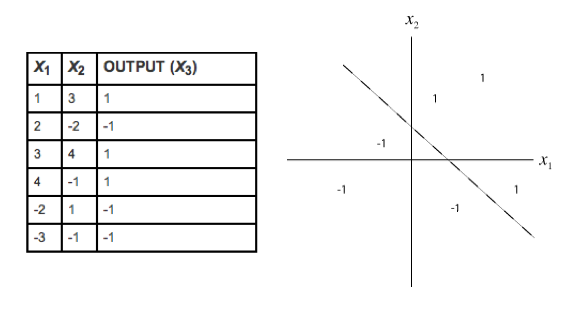
\includegraphics[scale=.6]{./images/decisionBoundary.png}
\caption{A classification task that can be solved by hand.}
\label{simpleTask}
\end{figure}

How do we design a neural network to solve this problem? First we build an appropriate network. It will have two input nodes and one output node. We make the output node a binary unit with upper bound 1, lower bound -1, and threshold 0. So the output node will output a 1 if weighted input is greater than 0, and -1 otherwise.

We now focus on the three adjustable parameters of the network: the two weight strengths $w_{1,3}$ and $w_{2,3}$, and the bias $b_3$ of the output node. A learning algorithm can learn this decision boundary automatically, but we can also just use algebra to find the right boundary.

To do this, we need to know how to make a network produce a particular decision boundary. The decision boundary in this case is the set of points in the $x_1 - x_2$ plane such that weighted input $n_3 = 0$. Points on one side of this line will produce  $n_3 > 0$, and so the output will be 1. Points on the other side of the line will produce an output of -1. (A geometric way of understanding what the decision boundary is included below). So we want to set the weights and bias so that this decision boundary has slope $-1$ and an $x_2$-intercept of $1$. The equation for the weighted input to neuron 3 is:
\begin{eqnarray*}
n_3 =  w_{1,3} x_1 + w_{2,3}  x_2 + b_3
\end{eqnarray*}
Since the set of points where $n_3$ is 0 is the decision boundary, we set $n_3$ to 0:
\begin{eqnarray*}
0 = x_1 w_{1,3} + x_2 w_{2,3} + b_3
\end{eqnarray*}
Now we solve for $x_2$:
\begin{eqnarray*}
x_2 = -\frac{w_{1,3}}{w_{2,3}} x_1  - \frac{b_3}{w_{2,3}}
\end{eqnarray*}
Notice that this is an equation for a line in the plane, that is, an equation of the form $y = mx + b$, where $m = -w_{1,3} / w_{2,3}$, and $b =  -b_3 / w_{2,3}$. To make this clear, here is the same equation, with boxes around the slope and intercept terms:
\begin{eqnarray*}
x_2 =  \boxed{-\frac{w_{1,3}}{ w_{2,3}}} x_1 - \boxed{\frac{b_3}{w_{2,3}}}
\end{eqnarray*}

Just by visual inspection of figure \ref{simpleTask}, we can see that the slope of a good decision line would be about -1, and a $x_2$-intercept of about 1. This is enough to build a network to solve the problem. The boxed values above correspond to the slope and $x_2$-intercept of the equation for the decision boundary. Our goal is to produce a network with a decision boundary like the one shown in figure \ref{simpleTask}, with slope -1 and $x_2$-intercept of 1. That is ,we want:
\begin{eqnarray*}
-\frac{w_{1,3}}{w_{2,3}} = -1 \\
-\frac{b_3 }{w_{2,3}} = 1 \\
\end{eqnarray*}
We can set the weight and bias values to do this in various ways. For example, we can set both weights to 1, so that the slope is -1. Then to set $x_2$-intercept to 1, we set $b_3$ to -1. So then our network parameters are:
\begin{eqnarray*}
w_{1,3}  = 1 \\
w_{2,3}  = 1 \\
b_3  = -1 \\
\end{eqnarray*}

This should give us the right results. Try building a network with these properties and see if it succeeds in the classification task  shown in figure \ref{simpleTask}.

So to summarize: the decision boundary, which separates the input space into different classes, shifts in two key ways: (1) its slope, determined by the ratio of the weights $-\frac{w_{1,3}}{w_{2,3}}$, and (2) its intercept, which is shifted left or right by the bias $b_3$, scaled by the weight $w_{2,3}$, as seen in the term $-\frac{b_3}{w_{23}}$.

\section{Geometric intuition about the decision boundary}

In the neural network discussed above, with two inputs and one output, the weighted input $n_3$ to the output node is given by the equation:
\[
n_3 = w_{1,3} x_1 + w_{2,3} x_2 + b_3
\]
The threshold for classification, that is the decision boundary, can be visualized as a horizontal plane, typically at $n_3 = 0$ (as in our example), which intersects the surface defined by the equation above. This intersection is normal (that is, perpendicular) to the vector $(w_{1,3}, w_{2,3})$. To see this, note that for any input $(p_1,p_2)$ for which $n_3 = 0$, $(w_{1,3}, w_{2,3}) \bullet  (p_1,p_2) = 0$, so the weight vector is orthogonal to any point on the decision boundary.

The bias $b_3$ shifts this plane vertically along the $z$-axis without affecting its orientation, while the weights determine the plane’s tilt. As you can see visually in the figure, inputs below the decision boundary will produce a net-input which is below threshold, while those above the decision boundary will produce a net-input which is above threshold.

This discussion provides a link between the discussion of regression surfaces and decision boundaries. As we can see here, the weighted input corresponds to a regression surface for a linear output node, and when we threshold that regression surface intersects another surface (corresponding to the threshold) and the result is a decision boundary.

\begin{figure}[h]
\centering
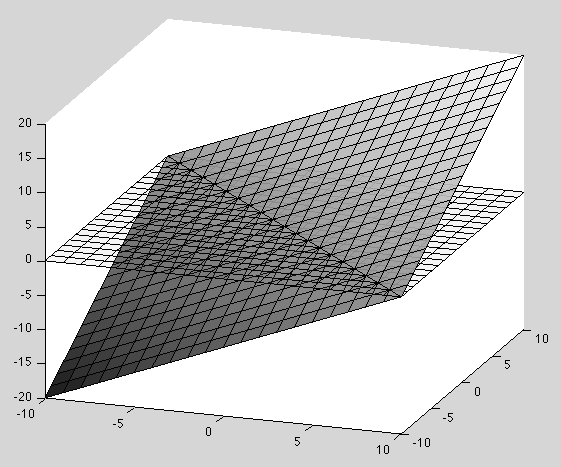
\includegraphics[scale=.4]{./images/decisionLinePlanes.png}
\caption{A decision boundary as the intersection of two surfaces.}
\label{decisionLineSurface}
\end{figure}


\chapter{New Material on Gradient Dynamics and Energy Functions}
\chapterauthor{Scott Hotton, Jeff Yoshimi}

% Break out sections. First, gradient dynamics. Do it intuitively. Explain how it is our main powerhouse for learning in the weight space, but also used to understand main dynamics using energy functions, as in Hopfield
% I have a fair number of notes with Scott on this to integrate as well.

\subsection{Dynamical systems from potential functions}

   A potential function is a smooth scalar field $V \colon \bf{R}^N \to 
\bf{R}$ which is used to perform gradient descent (see section 
\ref{sect_gradient_descent}). The gradient is a first order 
differential operator of functions from $\bf{R}^N$ to $\bf{R}$.  It is often
written as a vector with $N$ entries that are partial derivatives:
\begin{equation*}
   \nabla V(\mathbf{x}) = \left( \dfrac{\partial}{\partial x_1} V(\mathbf{x}),
\ldots, \dfrac{\partial}{\partial x_N} V(\mathbf{x}) \right)^T
\end{equation*}
The gradient tells us the direction in which the slope of the potential 
function is steepest, the direction in which $V$ increases the fastest.  The 
opposite direction is the one in which $V$ decreases the fastest.  

   A gradient dynamical system, also known as a gradient flow, is the solution 
to a differential equation that is obtained by using the gradient operator with
a potential function.  The state of the system is given by a point $\mathbf{x} 
\in \bf{R}^N$.  A gradient flow, is the solution to the differential equation 
obtained by setting the rate of change in $\mathbf{x}$ equal to the negative to 
the gradient of $V$ at $\mathbf{x}$:
\begin{equation}
   \dot{\mathbf{x}} = -\nabla V(\mathbf{x}) 
\end{equation}
No matter where $\mathbf{x}$ is in $\bf{R}^N$ it moves in the direction of
steepest descent of the potential function.  So the local minima of $V$ are 
attracting fixed points of a gradient flow.  All of the points in a small 
enough neighborhood of a local minimum of $V$ must converge to the local 
minimum.  The local maxima are repelling fixed points of a gradient flow.  All 
of the points in a small enough neighborhood of a local maximum (except for 
the local maximum itself) must move away from the local maximum.  

   At a local minimum or a local maximum there is no direction of steepest
descent so the gradient at these points has no direction, it is the zero 
vector.  In fact all of the fixed points of a gradient flow are either where 
the gradient is the zero vector or the gradient is undefined.  If the gradient 
is defined and not zero then $\mathbf{x}$ moves in the opposite direction of 
the gradient.  So long as the gradient is defined at the point $\mathbf{x}$ it
only does not move when the gradient is the zero vector.  The places where the 
gradient is zero or undefined are known as the critical points of the potential 
function.

   The matrix of second order partial derivatives
\begin{equation*}
-
\begin{pmatrix}
\dfrac{\partial^2}{\partial x_1^2}\, V(\mathbf{x}) &
\dfrac{\partial^2}{\partial x_1 \, \partial x_2}\, V(\mathbf{x}) &
\ldots & \dfrac{\partial^2}{\partial x_1 \partial x_N}\, V(\mathbf{x})  \\[4mm]
\dfrac{\partial^2}{\partial x_2 \, \partial x_1}\, V(\mathbf{x}) &
\dfrac{\partial^2}{\partial x_2^2}\, V(\mathbf{x}) &
\ldots & \dfrac{\partial^2}{\partial x_2\,  \partial x_N}\, V(\mathbf{x})  
\\[4mm]
   \vdots & \vdots & \ddots & \vdots \\[4mm]
\dfrac{\partial^2}{\partial x_N \, \partial x_1}\, V(\mathbf{x}) &
\dfrac{\partial^2}{\partial x_N \, \partial x_2}\, V(\mathbf{x}) &
\ldots & \dfrac{\partial^2}{\partial x_N^2}\, V(\mathbf{x})  \\[4mm]
\end{pmatrix}
\end{equation*}
is called the Hessian of $V$.  The entries of the $n^{\mathrm{th}}$ row of the
Hessian are the partial derivatives, with respect to $x_n$, of the entries of 
$-\nabla V(\mathbf{x})$.  The Hessian is a symmetric matrix because of the 
equality of mixed partial derivatives.
\begin{equation*}
\dfrac{\partial^2}{\partial x_j \, \partial x_k}\, V(\mathbf{x}) 
=
\dfrac{\partial^2}{\partial x_k \, \partial x_j}\, V(\mathbf{x}) 
\end{equation*}
for all $j$, $k \in \{1, \ldots, N\}$.  Since the Hessian is symmetric it does 
does not have complex conjugate pairs of eigenvalues.  All of its eigenvalues 
are real numbers. 

   If the determinant of the Hessian is zero then its called a degenerate
Hessian, otherwise its called nondegenerate.  Since the determinant of a
matrix is the product of its eigenvalues none of the eigenvalues of a 
nondegenerate Hessian can be zero.  When all of the second order partial 
derivatives are defined at a critical point of the potential function and the 
Hessian is nondegenerate then the critical point is either a minimum, a 
maximum, or a saddle point.  

   If all of the eigenvalues of the Hessian at a critical point are positive 
then the critical point is a local minimum.  If all of the eigenvalues of the 
Hessian at a critical point are negative then the critical point is a local 
maximum.  If some of the eigenvalues are positive and all of the other 
eigenvalues are negative then the critical point is a saddle point of the 
potential function.  This is a multidimensional version of the second 
derivative test from single variable calculus.  The eigenvectors for different 
eigenvalues of the Hessian are orthogonal.

   The attracting fixed points are the only attracting sets for a gradient 
flow.  For instance there are no attracting periodic orbits since we can not 
return to our starting point when we are always descending down the graph of 
$V$.  

   Aside from the fixed points, the orbits of a gradient flow are orthogonal to
each level hypersurface of $V$ that the orbits pass through.  The basin of 
attracting for the attracting fixed points are connected open sets in $\bf{R}^N$ 
with piecewise smooth boundaries.  Under a gradient flow every point in 
$\bf{R}^N$ is either in the basin of attraction of an attracting fixed point, in
the boundary of the basin of attraction, or it goes off to infinity.  The 
repelling fixed points and saddle nodes are located in the boundaries of the 
basins of attracting for the attracting fixed points.  

\begin{figure}[ht]
\centering
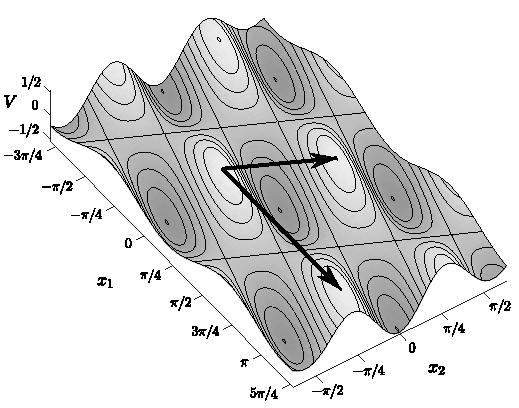
\includegraphics[scale=1.20]{./images/Gradient1.pdf}
\caption{The graph of the potential function $V( x_1, x_2)$ in equation 
\eqref{E:exampot} over the rectangular region $[-3\pi/4,5\pi/4] \times 
[-\pi/2,\pi/2]$.  The level curves of $V( x_1, x_2)$ are shown for 
multiples of $1/8$ in the interval $[-1,1]$.  They are typically closed 
curves that surround a local extremum but the level curves through the saddle 
points are a pair of straight lines.  The local minimum at $(\pi/4,0)^T$ has 
four local maximum and four saddle points as neighbors.  We can add $(\pi,0)^T$
to the neighboring local maximum at $(\pi/8,-\pi/4)^T$ to reach the neighboring
local maximum at $(9\pi/8,-\pi/4)^T$ and we can add $(\pi/4,\pi/2)^T$ to 
$(\pi/8,-\pi/4)^T$ to reach the neighboring local maximum at 
$(3\pi/8,\pi/4)^T$.  To get the fourth local maximum neighbor of 
$(\pi/4,0)^T$ we can add $(\pi,0)^T - (\pi/4,\pi/2)^T$ to $(\pi/8,-\pi/4)^T$.}
\label{F:exampot}  
\end{figure}

   We can demonstrate these facts with an example in two dimensions.  For
this example the potential function is:
\begin{equation}\label{E:exampot}
   V
\begin{pmatrix}
x_1 \\ x_2 
\end{pmatrix}
= -\frac{1}{4} \left( \sin(2 x_1 + 3 x_2) + \cos(4 x_2) \right)
\end{equation}
Since $V$ is defined in terms of the sine and cosine functions it is not 
surprising that it is a doubly periodic function of the plane.  In particular:
\begin{eqnarray*}
   V \left(
\begin{pmatrix}
x_1 \\ x_2
\end{pmatrix}
+
\begin{pmatrix}
\pi \\ 0
\end{pmatrix} \right)
= V
\begin{pmatrix}
x_1\\ x_2
\end{pmatrix} 
\qquad \mathrm{and} \qquad 
   V \left(
\begin{pmatrix}
x_1 \\ x_2 
\end{pmatrix}
+
\begin{pmatrix}
\pi/4 \\ \pi/2
\end{pmatrix} \right)
= V
\begin{pmatrix}
x_1\\ x_2
\end{pmatrix}
\end{eqnarray*}
for all $(x_1, x_2)^T \in \bf{R}^2$.  The double periodicity of $V$ can be seen
in Fig. \ref{F:exampot}.

\bigskip

\noindent
{\bf Exercise}: Confirm that $V$ has the periods $(\pi,0)^T$ and $(\pi/4, 
\pi/2)^T$.  \emph{Hint}: Use the fact that $\sin(x+2\pi)=\sin(x)$ and 
$\cos(x+2\pi) = \cos(x)$.

\bigskip

   The differential equation for the gradient flow in this example is:
\begin{equation*}
\begin{pmatrix}
\dot{x}_1 \\ \dot{x}_2 
\end{pmatrix}
=
-\nabla V
\begin{pmatrix}
x_1 \\ x_2 
\end{pmatrix}
=
\frac{1}{4} 
\begin{pmatrix}
2 \cos(2 x_1 + 3 x_2) \\ 3 \cos(2 x_1 + 3 x_2) - 4 \sin(4 x_2)
\end{pmatrix}
\end{equation*}
The fixed points of the gradient flow are the critical points of $V$.  These
are the solutions for $(x_1, x_2)^T$ in the equation:
\begin{equation*}
\begin{pmatrix}
0 \\ 0
\end{pmatrix}
=
\frac{1}{4} 
\begin{pmatrix}
2 \cos(2 x_1 + 3 x_2) \\ 3 \cos(2 x_1 + 3 x_2) - 4 \sin(4 x_2)
\end{pmatrix}
\end{equation*}
The critical points of $V$ are:
\begin{equation*}
\begin{pmatrix}
\pi/4 \\ 0
\end{pmatrix}
+ \frac{j}{2} 
\begin{pmatrix}
\pi \\ 0
\end{pmatrix}
+ \frac{k}{2}
\begin{pmatrix}
\pi/4 \\ \pi/2
\end{pmatrix}
=
\frac{\pi}{8}
\begin{pmatrix}
2+4j+k \\ 2k
\end{pmatrix}
\end{equation*}
for all $j$, $k \in \mathbf{Z}$.

\begin{figure}[ht]
\centering
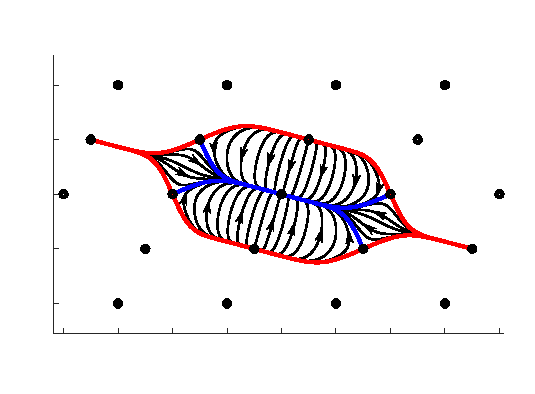
\includegraphics[scale=1.20]{./images/Gradient5.pdf}
\caption{xticks: \; $\displaystyle{-\frac{3\pi}{4}, \; -\frac{\pi}{2},\;  
-\frac{\pi}{4}, \; 0, \; \frac{\pi}{4}, \; \frac{\pi}{2}, \; \frac{3\pi}{4}, \; 
\pi, \; \frac{5}{4} \pi}$ \qquad
yticks: \; $\displaystyle{-\frac{\pi}{2}, \; -\frac{\pi}{4}, \; 0, \; 
\frac{\pi}{4}, \; \frac{\pi}{2}}$}
\end{figure}

\bigskip

\noindent
{\bf Exercise}: Confirm this equation and show that these are critical points 
of $V$.

\bigskip

   We can see from the right hand side of this equation that the set of 
critical points for $V$ forms a lattice in plane.  All of the integer multiples 
of the periods of $V$ (all of the integer multiples of $(\pi,0)^T$ and $(\pi/4, 
\pi/2)^T$) generates a sublattice.

   Within each unit cell of the sublattice there is one minimum for $V$, one 
maximum for $V$ and two saddle points for $V$.

\begin{figure}[ht]
\centering
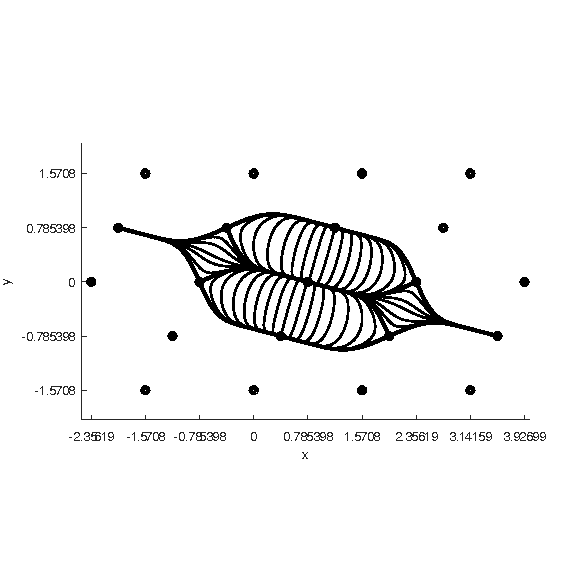
\includegraphics[scale=1.50]{./images/Gradient6.pdf}
\caption{Caption}
\end{figure}

\begin{figure}[ht]
\centering
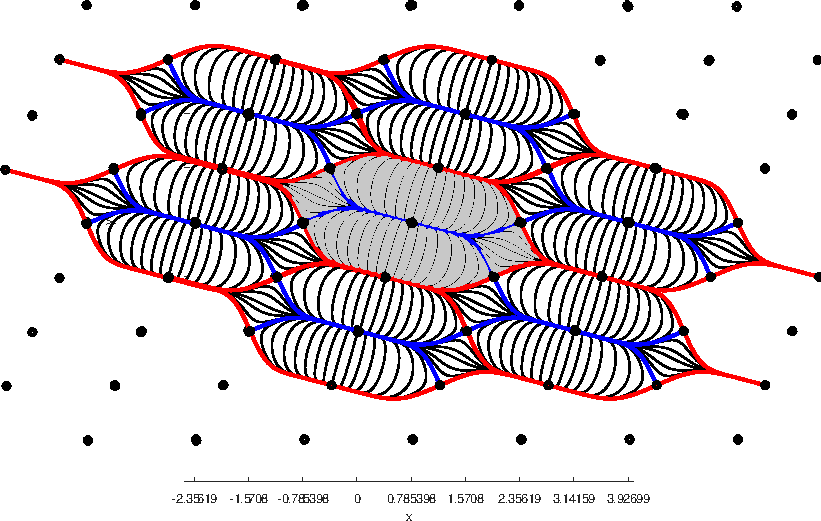
\includegraphics[scale=1.00]{./images/Gradient7.pdf}
\caption{Caption}
\end{figure}

\subsection{Hopfield network with two graded neurons}

   [Used different letters for pedagogy].  We denote the ``input'' of neuron 
$n$ by $x_n$ and the ``output'' by $y_n$.  The ``input-output relation'' (like 
an activation function) is:
\begin{equation*}
   y_n = g(x_n) = \frac{2}{\pi} 
                        \arctan\left( \frac{\pi}{2} \lambda x_n \right)
\end{equation*}
[This function is slightly different from how Hopfield did it in 1984 but it is 
how we did it our papers.]  Its inverse is:
\begin{equation*}
   x_n = g^{-1} (y_n) = \frac{2}{\pi\lambda} 
                        \tan\left( \frac{\pi}{2} y_n \right)
\end{equation*}

   Each stable fixed point will lie in a neighborhood of a vertex of an 
$N$-dimensional hypercube.  The hypercube will be the Cartesian product of the
closed interval $[-1,1] \subset \bf{R}$, \ie $[-1,1]^N$.  Its set of vertices
is $\{-1,1\}^N$.  The number of objects that a Hopfield can detect depends on
the number of neurons in the network.  The more objects we want the network to 
detect the more neurons we need to put in the network.  Experiments indicate
that the number of objects that can be reliably detected by a Hopfield network 
is about $15\%$ of the number of neurons.

   Our example will be a Hopfield network that can distinguish between two 
objects.  We let the vertices be opposite corners of the square
$\{-1,1\}^2$:
\begin{equation*}
\xi_1 = 
\begin{pmatrix}
\xi_{11} \\ \xi_{12}
\end{pmatrix}
=
\begin{pmatrix}
1 \\ -1
\end{pmatrix}
\qquad \mathrm{and} \qquad
\xi_2 = 
\begin{pmatrix}
\xi_{21} \\ \xi_{22}
\end{pmatrix}
=
\begin{pmatrix}
-1 \\ 1
\end{pmatrix}
\end{equation*}
From this we get the weights:
\begin{eqnarray*}
      w_{12} &=& \frac{1}{2} \; \xi_1 \bullet \xi_2
              =  \frac{1}{2} (1 \cdot (-1) + (-1) \cdot 1) = -1 \\
      w_{21} &=& \frac{1}{2} \; \xi_2 \bullet \xi_1
              =  \frac{1}{2} ((-1) \cdot 1 + 1 \cdot (-1)) = -1
\end{eqnarray*}
[I think there is a minor typo in the IJBC paper.  In the cogsci paper we 
referred to the IJBC paper on this.]  The self-weights are both $0$.

  Hopfield's potential function is 
\begin{eqnarray*}
V(x_1, x_2) = &-\,\displaystyle{\frac{1}{2}}& \left(
  \begin{matrix}\begin{pmatrix}y_1 & y_2\end{pmatrix}\\\mbox{}\end{matrix}
  \begin{pmatrix} w_{11} & w_{12} \\ w_{21} & w_{22} \end{pmatrix} 
  \begin{pmatrix} y_1 \\ y_2 \end{pmatrix} \right) \\
%% w_{11} y_1 y_1 + w_{12} y_1 y_2 + w_{21} y_2 y_1 + w_{22} y_2 y_2 \right) \\
&+& \left(\int_0^{y_1} g^{-1}(\chi) \, d\chi 
       + \int_0^{y_2} g^{-1}(\chi) \, d\chi\right) \\
&+& \left(I_1 y_1 + I_2 y_2 \right) \\
V(x_1, x_2) = &-\,\displaystyle{\frac{1}{2}}& \left(
 \begin{matrix}\begin{pmatrix}g(x_1) & g(x_2)\end{pmatrix}\\\mbox{}\end{matrix}
 \begin{pmatrix} 0 & -1 \\ -1 & 0 \end{pmatrix} 
 \begin{pmatrix} g(x_1) \\ g(x_2) \end{pmatrix} \right) \\
&+& \left(\int_0^{g(x_1)} g^{-1}(\chi) \, d\chi 
       + \int_0^{g(x_2)} g^{-1}(\chi) \, d\chi\right) \\
&+& \left(I_1 \, g(x_1) + I_2 \, g(x_2) \right) 
\end{eqnarray*}

\begin{eqnarray*}
V(x_1, x_2) = g(x_1) g(x_2) + \int_0^{g(x_1)} g^{-1}(\chi) \, d\chi 
                            + \int_0^{g(x_2)} g^{-1}(\chi) \, d\chi
             + I_1 \, g(x_1) + I_2 \, g(x_2) 
\end{eqnarray*}
To compute the integrals we compute the indefinite integral:
\begin{eqnarray*}
\int g^{-1}(\chi) \, d\chi  &=& \frac{2}{\pi\lambda} 
                        \int \tan\left( \frac{\pi}{2} \chi \right) \, d\chi \\
~ &=& \frac{2}{\pi\lambda} 
\left( -\frac{2}{\pi} \log\left( \left|\cos\left(\frac{\pi}{2}\chi \right)\right|\right)\right)
= -\frac{4}{\pi^2\lambda} 
\log\left( \left|\cos\left(\frac{\pi}{2}\chi \right)\right|\right)
\end{eqnarray*}
Therefore:
\begin{eqnarray*}
\int_0^{g(x_n)} g^{-1}(\chi) \, d\chi  &=& 
 -\frac{4}{\pi^2\lambda} \left.  \log\left( \left|\cos\left(\frac{\pi}{2}\chi 
\right)\right|\right)\right|_0^{g(x_n)} \\
~ &=& 
 -\frac{4}{\pi^2\lambda}  \log\left( \left|\cos\left(\frac{\pi}{2} g(x_n)
\right)\right|\right)
 +\frac{4}{\pi^2\lambda}  \log\left( \left|\cos(0) \right|\right) \\
~ &=& 
 -\frac{4}{\pi^2\lambda}  \log\left( \left|\cos\left(\arctan\left(
                        \left( \frac{\pi}{2} \lambda x_n \right)\right)\right)\right|\right) + 0
\end{eqnarray*}
We use trig identity for the composition of $\cos$ with $\arctan$.
Since the value of the composition of $\cos$ with $\arctan$ is positive 
everywhere we can drop the absolute signs.
\begin{eqnarray*}
\int_0^{g(x_n)} g^{-1}(\chi) \, d\chi  &=& -\frac{4}{\pi^2\lambda}  \log\left( 
\frac{1}{\sqrt{1 
+ \left(\displaystyle{\frac{\pi}{2}}\lambda x_n\right)^2}} \right) \\
~ &=& -\frac{4}{\pi^2\lambda}  \log\left( \left(1 
+ \left(\displaystyle{\frac{\pi}{2}}\lambda x_n\right)^2\right)^{-\displaystyle{\frac{1}{2}}} \right) \\
~ &=& \frac{2}{\pi^2\lambda}  \log\left( 1 
+ \left(\displaystyle{\frac{\pi}{2}}\lambda x_n\right)^2 \right)
\end{eqnarray*}
The potential function becomes:
\begin{eqnarray*}
V(x_1, x_2) = g(x_1) g(x_2) + 
\frac{2}{\pi^2\lambda} \left(
  \log\left( 1 + \left(\displaystyle{\frac{\pi}{2}}\lambda x_1\right)^2 \right)
+ \log\left( 1 + \left(\displaystyle{\frac{\pi}{2}}\lambda x_2\right)^2 \right)
\right) + I_1 \, g(x_1) + I_2 \, g(x_2) 
\end{eqnarray*}
Note that:
\begin{equation*}
g'(x_n) = \frac{2}{\pi} \dfrac{d}{d x_n} 
                        \arctan\left( \frac{\pi}{2} \lambda x_n \right)
= \frac{2}{\pi} \cdot
\frac{1}{1+ \left(\displaystyle{\frac{\pi}{2}}\lambda x_1\right)^2 }
\cdot \frac{\pi}{2} \lambda
= \frac{\lambda}{1+ \left(\displaystyle{\frac{\pi}{2}}\lambda x_1\right)^2 } 
\end{equation*}
So that
\begin{equation*}
1+ \left(\displaystyle{\frac{\pi}{2}}\lambda x_1\right)^2 = 
\frac{\lambda}{g'(x_n)}
\end{equation*}
The potential function becomes:
\begin{eqnarray*}
V(x_1, x_2) &=& g(x_1) g(x_2) + 
\frac{2}{\pi^2\lambda} \left(
\log\left( \frac{\lambda}{g'(x_1)} \right)
+
\log\left( \frac{\lambda}{g'(x_2)} \right) \right)
+ I_1 \, g(x_1) + I_2 \, g(x_2)  \\
~  &=& g(x_1) g(x_2) + 
\frac{2}{\pi^2\lambda} 
\log\left( \frac{\lambda^2}{g'(x_1) g'(x_2)} \right)
+ I_1 \, g(x_1) + I_2 \, g(x_2)  
\end{eqnarray*}

  To get the negative gradient of the potential we begin with the partial 
derivative with respect to $x_1$: gradient:
\begin{eqnarray*}
\dfrac{dV}{d x_1}(x_1, x_2) &=& g'(x_1) g(x_2) - \frac{2}{\pi^2 \lambda}
\cdot \frac{g''(x_1)}{g'(x_1)}
+ I_1 \, g'(x_1) 
\end{eqnarray*}
Note that:
\begin{eqnarray*}
g''(x_1) &=& \dfrac{d}{d x_1} g'(x_1) = \dfrac{d}{d x_1} 
\frac{\lambda}{1+ \left(\displaystyle{\frac{\pi}{2}}\lambda x_1\right)^2 } \\
~ &=& - \frac{\lambda}{\left(1+ 
\left(\displaystyle{\frac{\pi}{2}}\lambda x_1\right)^2 \right)^2} \cdot 
\left(\frac{\pi \lambda}{2}\right)^2 x_1 \\
 ~ &=& -\frac{\pi^2 \lambda}{4} \, x_1 \left( 
\frac{\lambda}{1+ \left(\displaystyle{\frac{\pi}{2}}\lambda x_1\right)^2 } 
\right)^2 = -\frac{\pi^2 \lambda}{4} \, x_1 g'(x_1)^2
\end{eqnarray*}
Substituting into $dV/dx_1$ gives:
\begin{eqnarray*}
\dfrac{dV}{d x_1}(x_1, x_2) &=& g'(x_1) g(x_2) - \frac{2}{\pi^2 \lambda}
\cdot \left(-\frac{\pi^2 \lambda}{4} \, x_1 \cdot \frac{g'(x_1)^2}{g'(x_1)} \right)
+ I_1 \, g'(x_1) \\
~ &=& g'(x_1) g(x_2) + \frac{1}{2} x_1 g'(x_1) + I_1 \, g'(x_1) \\
~ &=& g'(x_1) \left(\frac{1}{2} x_1  + g(x_2) + I_1\right) 
\end{eqnarray*}
We get $dV/dx_2$ by reversing the subscripts $1$ and $2$.  The ODE for 
gradient descent becomes:
\begin{eqnarray*}
\begin{pmatrix}
\dot{x}_1 \\ \dot{x}_2 
\end{pmatrix}
=
\begin{pmatrix}
g'(x_1) \cdot \left( (1/2) \, x_1  + g(x_2) + I_1\right)  \\[2mm]
g'(x_2) \cdot \left( (1/2) \,  x_2  + g(x_1) + I_2\right) 
\end{pmatrix}
\end{eqnarray*}
If we drop the factors $g'(x_1)$ and $g'(x_2)$ we get the Hopfield's ODE:
\begin{eqnarray*}
\begin{pmatrix}
\dot{x}_1 \\ \dot{x}_2 
\end{pmatrix}
=
\begin{pmatrix}
 (1/2) \, x_1  + g(x_2) + I_1  \\[2mm]
 (1/2) \,  x_2  + g(x_1) + I_2 
\end{pmatrix}
\end{eqnarray*}
Except for the factor $1/2$ which is probably comes from a typo in typesetting.

\chapter{New Material LMS and Backprop}
\chapterauthor{Jeff Yoshimi}

\subsection{Derivation of the LMS rule}

% Add this material and notes from lecture
The nice thing about LMS is we can directly interpret it in terms of Goldilocks.

All this can be shown using calculus. It's kind of amazing to turn the crank on the calculus, and see how it all works out giving us the rule above, with all the intuitive meaning. Run through the calculus, and we get our rule, which we saw above makes sense!

Conceptually, we are using the derivative of the error space. Since it's multi-dimensional, we call the derivative a gradient in this case. The gradient is a vector that points in the direction of change. 

We want to change the weight so that error is reduced. Let's leave the bias out for now. Then we are taking the  derivative of this error function:

\begin{eqnarray*}
E = (t - a_2)^2  =  (t - ( a_1 w_{1,2} + b_2))^2  =  (t -  a_1 w_{1,2} -  b_2)^2 
\end{eqnarray*}
with respect to a weight $w_{1,2}$.  Using the chain rule (derivative of the outside part applied to the inside part, times the derivative of the inside part), and substituting, we get

\begin{eqnarray*}
\frac{dE}{dw_{1,2}} = 2 (t - a_1 w_{1,2} - b_2) (-a_1) =  -2 a_1 (t - a_1 w_{1,2} - b_2) =  -2 a_1 (t - a_2)
\end{eqnarray*}

And since $t -  a_2$ is error $e_2$ we get

\begin{eqnarray*}
\frac{dE}{dw_{1,2}} = -2 e_2 a_1
\end{eqnarray*}

This says that the change in error with respect to the weight is given by error times source activation times a constant. The 2 can be ignored, since we can think of it as being absorbed into the learning rate. Also, this gradient points in the direction of error increasing. But we want to go in the opposite direction, so that error is reduced (this is gradient descent, not gradient ascent). So we multiply the gradient by $-1$, changing its sign. And so our learning rule is 

\begin{eqnarray*}
\Delta w_{1,2}  =  \epsilon a_1 e_2  = \epsilon a_1 (t - a_2)
\end{eqnarray*} 

Of course this generalizes, and so our general learning rule for weights is:
\begin{eqnarray*}
\Delta w_{i,j}  =  \epsilon a_i (t_j - a_j)
\end{eqnarray*} 

As an exercise, try deriving the rule for bias. Again the error function is

\begin{eqnarray*}
E =  (t - ( a_1 w_{1,2} + b_2))^2 
\end{eqnarray*}
but in this case we want to find $\frac{dE}{db_{2}}$.

Now let's add in the activation function $f$ and derive the weight-update rule. Now the error function is:

\begin{eqnarray*}
E =  (t - f(a_1w_{1,2} + b_2))^2   
\end{eqnarray*}

and so

\begin{eqnarray*}
\frac{dE}{dw_{1,2}} = 2 (t - f(a_1w_{1,2} + b_2)) f'(a_1w_{1,2} + b_2) a_1 
\end{eqnarray*}

Subbing in $a_2 = f(a_1w_{1,2} + b_2))$, and recalling $n_2 = w_{1,2} + b_2$  and $t - a_2 = e_2$ 

\begin{eqnarray*}
\frac{dE}{dw_{1,2}}  = 2 e_2 f'(n_2) a_1 
\end{eqnarray*}

So the learning rule for weights is:
\begin{eqnarray*}
\Delta w_{i,j}  =  \epsilon a_i e_j f'(n_j)
\end{eqnarray*} 

This is the same as before, but multiplied by the derivative of the activation function applied to to the net input (the weighted input to the node). We discuss this more below. 

Note that the derivative of the activation function $f'$ is like a free parameter in this formula. Whatever your activation function $f$ is, to use gradient descent we just plug in $f'$ and we can do gradient descent. Situations like this allow backprop to be automated in a sense. But note that some derivatives have problems, like being undefined or 0, which effectively turns off update.

Intuitively, the idea is to scale the rate of weight change by how much the activation function is changing things. So when the activation function is changing things a lot, we want the weight to change a lot too. When it changes things very little, the derivative is small and so we change the weight less. It doesn't matter as much. Also note that if the derivative is 0, then learning stops. That can be a problem with piecewise linear and relu activation functions, and is why the threshold activation function can't be used at all. Again see below.

\section{Vector approach to LMS}

In the scalar approach to LMS we multiply a single output error (target - output) by source activation. Now we have a vector of errors times a vector of source activations. But how to deal with indexing?  The algorithm is ultimately a variant on Hebb, so we already have a template for thinking about it (see the discussion of the vectorized Hebb rule)
% Reference the new material on Hebb here

The error part itself is easy, first we do target - output using elementwise subtraction: $\mathbf{t} - \mathbf{a}_{\text{out}}$. To multiply these errors times source activations, we do the same thing as in Hebb: we multiply an $m \times  1$ column output errors times a $1 \times  n$ row of source activations to get an $m \times n$ matrix of weight deltas. Then we scale that by learning rate, and add to the weight matrix. (There remains the issue of the bias, and any activation functions on the output, but we're starting simple.) So, the vectorized rule is
\begin{eqnarray*}
\Delta \mathbf{W}  =  \epsilon (\mathbf{t} - \mathbf{a}_{\text{out}}) \mathbf{a}_{\text{in}}^T
\end{eqnarray*}
Remember, by default all vectors in bold face are column vectors. So this is a column vector (the error $\mathbf{t} - \mathbf{a}_{\text{out}}$) times a row vector (the input activations) which produces a matrix in the same shape as the weight matrix.

Consider the network shown in figure \ref{lms_vector_pre}.

\begin{figure}[h]
\centering
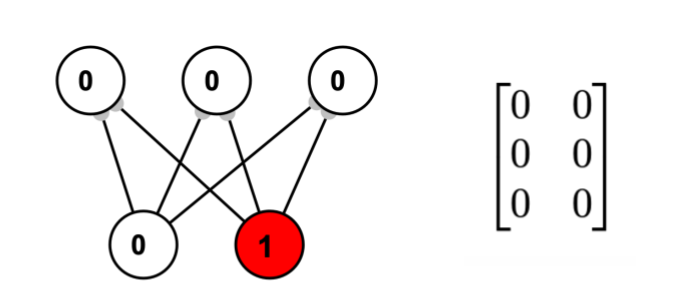
\includegraphics[width=0.55\textwidth]{images/vectorLMSBeforeTrain.png}
\caption[Jeff Yoshimi.]{A network with empty weights. We want it to learn to associate the input vector $(0,1)$ with the output vector $(1,0,1)$, but right now the weights are all zero so it just outputs $(0,0,0)$. }
\label{lms_vector_pre}
\end{figure}

Remember, the weight matrix is a 3x2 matrix  (``target-source''), which we are treating as all zero in this example. Each row is a fan-in of an output node, and the columns are fan-outs of input nodes. Our template for thinking about this is to imagine inputs coming up from the bottom, and dotting with the fan-in weight vectors to produce outputs.

Our values are
\begin{equation*}
\epsilon = 1 \; \; \\
\mathbf{a}_{\text{in}} = \begin{bmatrix} 0 \\ 1 \end{bmatrix} \\
\mathbf{t} = \begin{bmatrix} 1 \\ 0 \\ 1 \end{bmatrix}
\mathbf{a}_{\text{out}} = \begin{bmatrix} 0 \\ 0 \\ 0 \end{bmatrix}
\end{equation*}

Then the equation is learning rate times error times input transposed:

\begin{align*}
\Delta \mathbf{W}  = 1
\begin{bmatrix} 1 \\ 0 \\ 1 \end{bmatrix} 
\begin{bmatrix} 0 & 1 \end{bmatrix} 
= \begin{bmatrix} 1 \cdot 0 & 1 \cdot 1 \\ 0 \cdot 0 & 0 \cdot 1 \\ 1 \cdot 0 & 1 \cdot 1 \end{bmatrix} 
= \begin{bmatrix} 0 & 1 \\ 0 & 0 \\  0 & 1  \end{bmatrix}
\end{align*}

So we get

\begin{align*}
\mathbf{W} + \Delta \mathbf{W}  =
\begin{bmatrix} 0 & 0 \\ 0 & 0 \\  0  & 0  \end{bmatrix} +
\begin{bmatrix} 0 & 1 \\ 0 & 0 \\  0  & 1  \end{bmatrix} =
\begin{bmatrix} 0 & 1 \\ 0 & 0 \\  0  & 1  \end{bmatrix}
\end{align*}

And again, keeping in mind that rows are fan-in of output and columns are fan-out of input we get figure \ref{lms_vector_2}.

\begin{figure}[h]
\centering
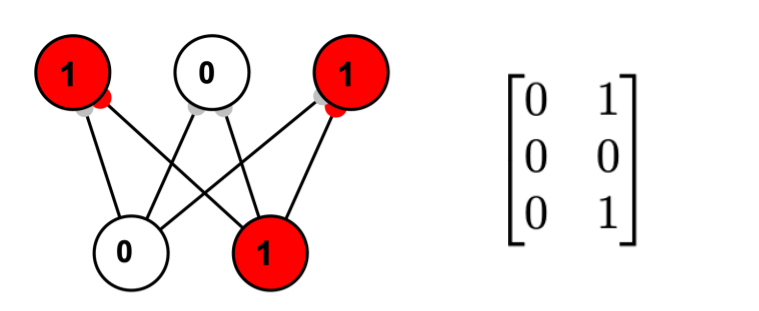
\includegraphics[width=0.55\textwidth]{images/vectorLMSAfterTrain.png}
\caption[Jeff Yoshimi.]{The network after training}
\label{lms_vector_2}
\end{figure}

We can now check that it works. Remember, think of the column vector on the right as ``entering'' from below, and dotting with each fan-in weight vector (each row of the matrix) to produce the output. SSE has gone to 0 in a single time step.

\begin{align*}
\begin{bmatrix} 0 & 1 \\ 0 & 0 \\  0  & 1  \end{bmatrix}
\begin{bmatrix} 0 \\ 1 \end{bmatrix}
= \begin{bmatrix} 1 \\ 0 \\ 1  \end{bmatrix}
\end{align*}

% Add exercizes here, use Mak and David examples.
So now I suggest you try some examples of your own. Come up with your own training set, apply the rule and see if you can run this a few times. 

\subsection{Bias}

To add bias updates in, we just vectorize the bias update rule, which has the same form as the scalar rule, since it's just elementwise.

\begin{eqnarray*}
\Delta \mathbf{b}  =  \epsilon (\mathbf{t} - \mathbf{a}_{out})
\end{eqnarray*}

So at each iteration, we change the bias vector just in the direction of the error vector. Remember goldilocks. When things are too hot, cool them down. Etc.

\subsection{Activation functions}

The full LMS rule also involves a derivative on the activation function. These derivatives can be understood pretty intuitively if we look at those again. See figure \ref{derivativesActFunctions}. The derivative for the threshold function is 0 everywhere except at the threshold where it is undefined (this was a problem for Rosenblatt). The derivative for the piecewise linear is 0 above and below the upper and lower bounds and the slope (usually 1) of the function in between those bounds. For the sigmoid it's close to what it is for piecewise linear, approaching 1 as net input is large or small and the slope at the inflection point in the middle, but we do need a formula for it.

\begin{figure}[h]
\centering
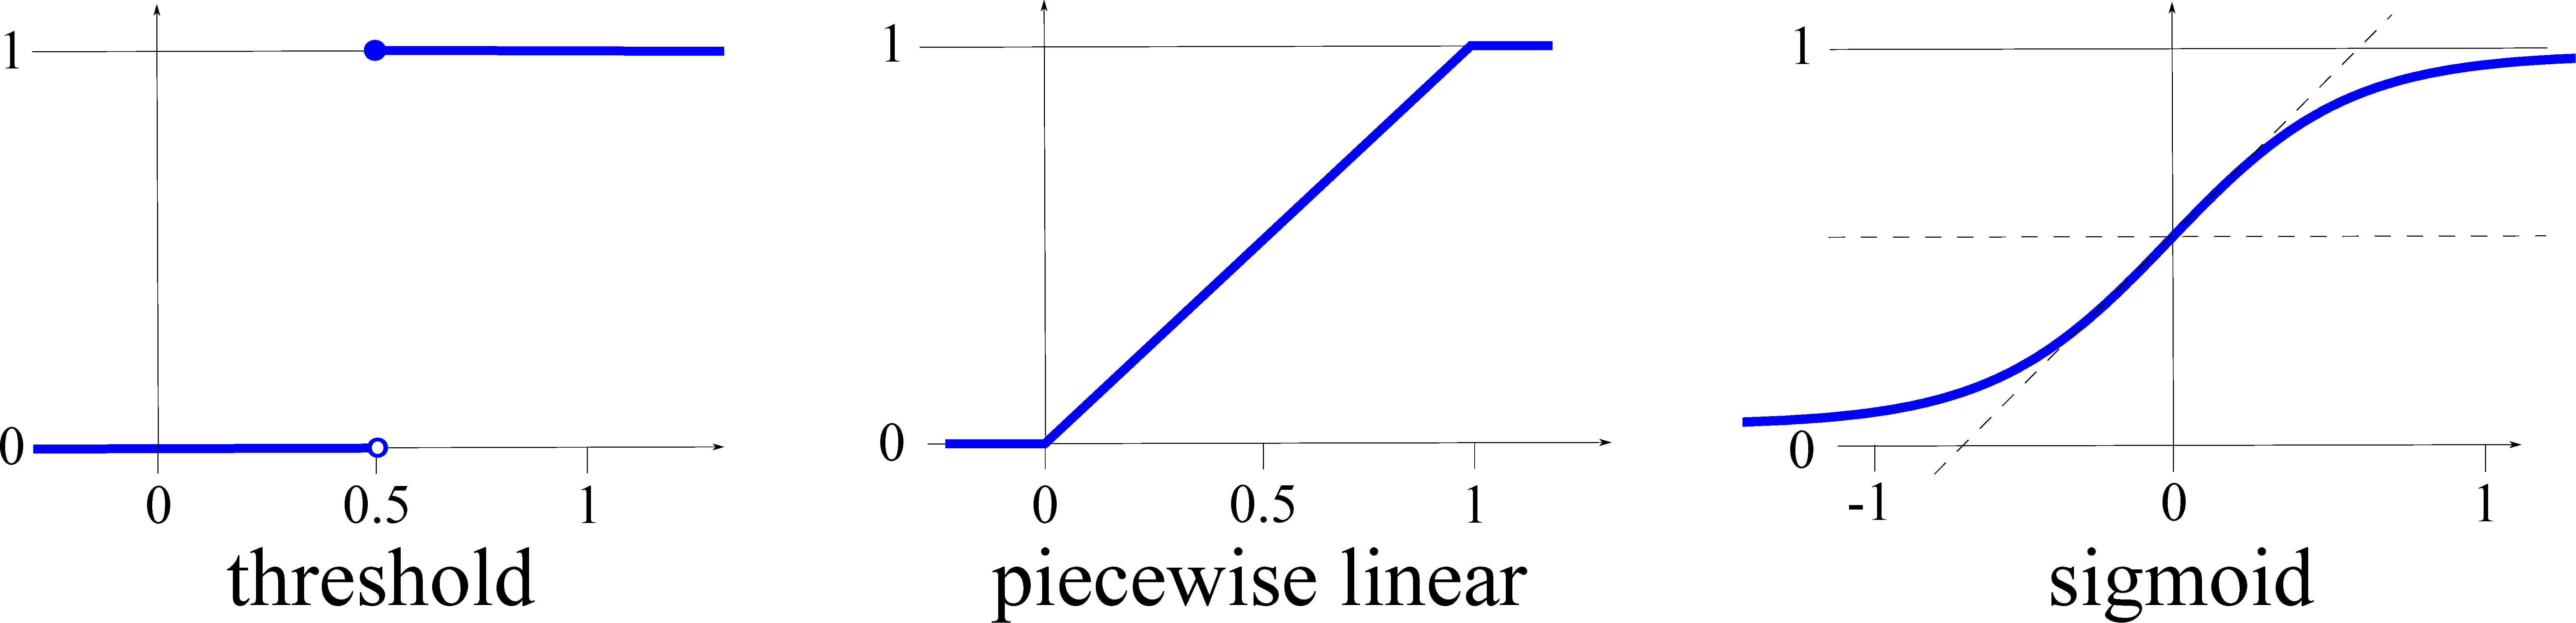
\includegraphics[width=0.75\textwidth]{images/graph_binary.pdf}
\caption[Jeff Yoshimi.]{The activation functions. The derivative is either 0 or the slope or close to the slope in most cases. }
\label{derivativesActFunctions}
\end{figure}

So how to work this into the LMS error update?

First, recall from chapter \extref{ch_act_functions} that the weighted input to a node $j$ is denoted $n_j$. This is the same as the activation of a linear unit. Its weights times input activations plus a bias. An activation function $f$ then transformed this weighted inputs, so that $a_j = f(n_j)$. When we incorporate activation functions we have to keep $a_j$ and $n_j$ separate so just get that clear before moving on.

Ok, and recall from the derivation that error update with an activation function involves the same as before multiplied by with the derivative of the activation function applied to the net input. Intuitively it's like we scale the error that we use to scale the weights and biases with a factor corresponding to how much the activation function changes things.\footnote{This is a problem with RELU, known as the ``dying Relu" problem.}  It's also why Rosenbatt's perception was limited; binary are 0 derivative everywhere so their weights never change using this rule, and so he had to come up with a kind of ad hoc solution.

So the full rule for weights is

\begin{eqnarray*}
\Delta w_{i,j}  =  \epsilon a_i (t_j - a_j) f' (n_j)
\end{eqnarray*}

And the full rule for biases is 

\begin{eqnarray*}
\Delta b_{j}  =  \epsilon b_j (t_j - a_j) f' (n_j)
\end{eqnarray*}

Do both of these at each time step to update the network.

\subsection{The Vectorized LMS rule with Activation Functions}

% TODO: This is now a bit redundant with the material above
To express this all in vectorized form we have to take the individual entries and see what happens when we express the ideas using vectors.  Again it's a kind of bookkeeping exercise. Here is what we get.

\begin{eqnarray*}
\Delta \mathbf{W}  =  \epsilon ((\mathbf{t} - \mathbf{a}_{\text{out}}) \odot f'( \mathbf{n}_{\text{out}})) \mathbf{a}_{\text{in}}^T
\end{eqnarray*}
Where $\odot$ is component-wise or Hadamard product (see section X). That is, we take a column vector of errors $\mathbf{t} - \mathbf{a}_{\text{out}}$, and then component-wise multiply by a vector of derivatives applied to weighted inputs $f'( \mathbf{n}_{\text{out}})$, effectively scaling each component of the error by the corresponding derivative. 

We then matrix multiply the resulting column vector of scaled errors by a row vector of source activations $ \mathbf{a}_{\text{in}}^T$, and the result is a matrix of weight deltas with the right shape. This is sometimes called an ``outer product'', where a $n_{out} \times 1$ scaled error vector is multiplied by a  $1 \times n_{in}$ vector if input activations, producing an $n_{out} \times n_{in}$ matrix of weight deltas. The whole thing is then scaled by the learning rate $\epsilon$.

For the vector of biases we have:

\begin{eqnarray*}
\Delta \mathbf{b}  =  \epsilon (\mathbf{t} - \mathbf{a}_{\text{out}}) \odot f'( \mathbf{n}_{\text{out}})
\end{eqnarray*}
We're basically just changing the biases by the error vector scaled by the derivatives, and leaving out the step where we consider input activations.

\subsection{Batch version of the rule}

In many neural network implementations, computations are applied to batches of data. In this setup, inputs are not passed through a network as single column vectors, but whole batches are (see section X). This is much more computationally efficient and leverages the power of modern hardware like GPUs which are optimized for matrix computations.  It thus helps to be able to think in terms of batches being processed.

By convention, batches are matrices where the rows are input vectors, target vectors, etc., and so they have shape $B \times n$, where $B$ is the batch size and $n$ is the size of the relevant vector. This is nice and easy to think about; basically the batches are little input table, target tables, output tables, etc (see section X).

For a single linear network with one weight layer $\mathbf{W}$, the forward pass is computed like this:

\begin{eqnarray}
\mathbf{Y} = \mathbf{X} \mathbf{W}^T
\end{eqnarray}
where $\mathbf{X}$ is the batch of inputs and has a shape of $B \times n_{in}$, where $B$ is the batch size and $n_{in}$ is the number of nodes in the input layer. Again, it's a kind of input table. $\mathbf{W}$ is transposed so that we get a shape of $n_{in} \times n_{out}$. This is the source-target representation we emphasized in the scalar track (see section X), where columns correspond to fan-in weight vectors. This allows us to think of the product as a bunch of vector-matrix multiplications (or ``right multiplications'' since the matrix is on the right), where we peel off the rows of the input table $\mathbf{X}$ one at a time, multiply them by the weight matrix (dotting the rows with each column of $\mathbf{W}^T$), in each case producing an output vector in $\mathbf{Y}$. As we move down the rows of the input table we stack up rows of the output table or output batch $\mathbf{Y}$, which has a shape of $B \times n_{out}$.

To calculate error, we compare the output $\mathbf{Y}$ with a ``target table" (a batch of target values). Subtracting the target values from the output activations gives us an error matrix:
\begin{eqnarray}
\mathbf{E} = \mathbf{Y} - \text{targets}
\end{eqnarray}
where $\mathbf{E}$ also has a shape of $B \times n_{out}$.

Now for backprop. The gradient of the loss with respect to the output activations in $\mathbf{Y}$ is proportional to the error matrix $\mathbf{E}$. If we are averaging the loss over the batch, this outer gradient becomes:

\begin{eqnarray}
\frac{\partial \text{Loss}}{\partial \mathbf{Y}} = \frac{1}{B} \mathbf{E}
\end{eqnarray}

To update the weights, we use the chain rule to express the gradient of the loss with respect to the weights $\mathbf{W}$ as follows:

\begin{eqnarray}
\frac{\partial \text{Loss}}{\partial \mathbf{W}} = \frac{\partial \text{Loss}}{\partial \mathbf{Y}} \cdot \frac{\partial \mathbf{Y}}{\partial \mathbf{W}}
\end{eqnarray}

Since we have $\frac{\partial \text{Loss}}{\partial \mathbf{Y}} = \frac{1}{B} \mathbf{E}$, we then calculate $\frac{\partial \mathbf{Y}}{\partial \mathbf{W}}$ by noting that $\mathbf{Y} = \mathbf{X} \mathbf{W}^T$. This is a matrix version of a familiar scalar derivative like $dy/dw(y = xw) = x$, and in a similar way the derivative of the matrix version is $\mathbf{X}$. 

Combining these derivatives gives us:

\begin{eqnarray}
\frac{\partial \text{Loss}}{\partial \mathbf{W}} = \frac{1}{B} \mathbf{E}^T \mathbf{X}
\end{eqnarray}
Here, $\mathbf{E}^T$ has a shape of $n_{out} \times B$, and $\mathbf{X}$ has a shape of $B \times n_{in}$. Multiplying these gives an $n_{out} \times n_{in}$ matrix, which aligns with the shape of $\mathbf{W}$ and represents the weight updates.

% Make this a separate section on decomposing this kind of product into a sum of outer products?
A brief interlude: this can be a bit confusing but one helpful way to think of it is as a sum of outer products of the kind we saw in the vectorized hebb rule and the vectorized (but not batched) LMS rule. The matrix product $\mathbf{E}^T \mathbf{X}$ can be expanded as a sum of outer products of each error vector $\mathbf{e}_i$ (rows of $\mathbf{E}$) and input vectors $\mathbf{x}_i$ (rows of $\mathbf{X}$). Now when we index like that, this identity holds:
\begin{eqnarray}
\mathbf{E}^T \mathbf{X} = \sum_{i=1}^{B} \mathbf{e}_i^T \mathbf{x}_i
\end{eqnarray}
which gives us a sum of outer products.

For example, suppose we have
\begin{eqnarray*}
\mathbf{E} = \begin{pmatrix} 1 & 2 \\ 3 & 4 \end{pmatrix}, \quad \mathbf{X} = \begin{pmatrix} 2 & 3 \\ 4 & 5 \end{pmatrix}
\end{eqnarray*}
These are both row-based matrices. $\mathbf{E}$ has errors as rows (what we sometimes call ``row errors'') and $\mathbf{X}$ has inputs as rows. So it's a nice familiar way to conceptualize things. Then we can expand $\mathbf{E}^T \mathbf{X}$ in a way that makes it clear we are taking outer products of these and summing them to get the weight deltas:
\begin{eqnarray*}
\mathbf{E}^T \mathbf{X} = \mathbf{e}_1^T \mathbf{x}_1 + \mathbf{e}_2^T \mathbf{x}_2 = \begin{pmatrix} 1 \\ 2 \end{pmatrix} \begin{pmatrix} 2 & 3 \end{pmatrix} + \begin{pmatrix} 3 \\ 4 \end{pmatrix} \begin{pmatrix} 4 & 5 \end{pmatrix} = \begin{pmatrix} 2 & 3 \\ 4 & 6 \end{pmatrix} + \begin{pmatrix} 12 & 15 \\ 16 & 20 \end{pmatrix} = \begin{pmatrix} 14 & 18 \\ 20 & 26 \end{pmatrix}
\end{eqnarray*}

Now we can state the weight update rule for batched LMS without bias or activation rules. Using the learning rate $\epsilon$, and remembering that we are doing gradient descent so that the derivative has to be multiplied by $-1$, the weight change for the matrix in the batch case is:

\begin{eqnarray}
\Delta \mathbf{W} =  - \epsilon \frac{1}{B} \mathbf{E}^T \mathbf{X}
\end{eqnarray}
   
\subsection{Backprop and Automatic Differentiation}

As we move to learning rules for more than one weight layer, it is harder to interpret things directly, but we can abstractly understand them and also conceive of them in a kind of modular way, building off chain rules like the one above, 
\begin{eqnarray}
\frac{\partial \text{Loss}}{\partial \mathbf{W}} = \frac{\partial \text{Loss}}{\partial \mathbf{Y}} \cdot \frac{\partial \mathbf{Y}}{\partial \mathbf{W}}
\end{eqnarray}
Just with potentially way more steps than that.
% Integrate classroom notes and images on this

\chapter{New Material on Hopfield}
\chapterauthor{Scott Hotton, Jeff Yoshimi}

% See Week9_RNN.txt
% Add RBM info at bottom or in a new doc
% Add references on the types of update, Amit and original Hopfield (async/sync, but not sequential I don't think)

\section{New Material on Hopfield Networks}

% Basically he did these things
% First, mapped from binary to bipolar using the 2v-1 trick, to get the nice properties we talked about while dealing with nice binary patterns
% Second used symmetric weight matrices which allow lyapunov functions
% Third used a custom update rule

   For a discrete Hopfield network we denote the input of neuron $n$ by $x_n$ 
and the output by $y_n$.  Neuron states are updated using an input-output 
relation.  If the input to neuron $n$ is below the threshold $U_n$ then the
output from neuron $N$ is $0$, otherwise the output is $1$.  This input-output
relation can be concisely expressed as:
\begin{equation}\label{E:hopIO}
   y_n(t+1) = 
\left\{
\begin{array}{ll}
0 & \mbox{if} \quad x_n(t) \leq U_n   \\
1 & \mathrm{otherwise} 
\end{array}\right.
\end{equation}
The threshold $U_n$ is often set to $0$ for all of the nodes.  So $y_n(t+1)$ is 
$0$ if $x(t)$ is not positive and it $1$ if $x(t)$ is positive.  

   The output of each neuron is an input for every neuron aside from itself.
The inputs are a linear combination of the state vector $(y_1, y_2, \ldots,
y_N)^T$ plus an input vector from the external environment.  The contribution
from each neuron is given by the weight matrix for the network.  The weight
matrix is is obtained as follows.

   Some of the vertices of an $N$ dimensional hypercube are chosen to be the 
attracting fixed points for a network.  The vertex for the $n^{\mathrm{th}}$ 
object is denoted by 
\begin{equation*}
\boldsymbol{p}_n =
\begin{pmatrix}
p_{1n} \\ p_{2n} \\ \vdots \\ p_{Nn}
\end{pmatrix}
\end{equation*}
for $n = 1,2, \ldots, N$.  In order for $\boldsymbol{p}_n$ to be a vertex
of the hypercube $[0,1]^N$ we need $p_{jn}$ to be $0$ or $1$ for all $j$, $n 
\in \{1, \ldots, N\}$.

   In a Hopfield network the weight of a neuron to itself is always $0$.
Otherwise the general formula the weights is:
\begin{equation}\label{E:hopweights}
w_{jk} = \sum_{n=1}^N (2 p_{nj} - 1)(2 p_{nk} - 1) 
\end{equation}
for all $j$, $k \in \{1, \ldots, N\}$ and $j \neq k$.  It follows that 
$w_{jk} = w_{kj}$ for all $j$, $k \in \{1, \ldots, N\}$ and that the weight 
matrix for a Hopfield network is symmetric.  

   The input to each neuron is a weighted combination of the activations for 
all of the other neurons plus a term for the external environment which we 
assume here is constant.  We let $I_n$ denote the external input and 
$(I_1, I_2, \ldots, I_n)^T$ denote the vector of fixed inputs to the $N$ nodes 
in the neural network.  The inputs to the neurons at time $t$ can be expressed
concisely as:
\begin{equation}\label{E:hopinput}
\begin{pmatrix}
x_1(t) \\  x_2(t) \\ \vdots \\ x_N(t)
\end{pmatrix}
 = 
 \begin{pmatrix} 
     0      & w_{12} & \cdots & w_{1N} \\ 
     w_{12} &   0    & \cdots & w_{2N} \\ 
     \vdots & \vdots & \ddots & \vdots \\ 
     w_{1N} & w_{2N} & \cdots &   0  
 \end{pmatrix} 
 \begin{pmatrix} 
     y_1(t) \\ y_2(t) \\ \vdots \\ y_N(t) 
  \end{pmatrix} 
     +
\begin{pmatrix}
I_1 \\  I_2 \\ \vdots \\ I_N
\end{pmatrix}
\end{equation}
A Hopfield network operates by successively applying rules \eqref{E:hopinput} 
and \eqref{E:hopIO}.

\subsection{Types of Update}

   The rules \eqref{E:hopinput} and \eqref{E:hopIO} can be apply synchronously
or asynchronously.  With synchronous update rules \eqref{E:hopinput} and 
\eqref{E:hopIO} are successively applied to all of the neurons at the same 
time.  For a fixed input vector this gives us a function from the state space 
to itself.  By iterating this function we obtain a dynamical system on the 
neural network's state space.  With synchronous update the states chosen to be
the attracting fixed points do become attracting fixed points for the 
appropriate inputs.

   Synchronous update is not used very often because it allows the neural
network to become stuck in oscillations when more than one object is present 
in the environment.  So it can not decide whether an object is present or not.
Instead of updating all of the neurons in a Hopfield network at the same time 
we can update them one at a time.  Hopfield proposed two ways to do this.  One 
way is to go through each of neurons in the network in some fixed order.  This 
is called \emph{sequential update}.  We choose a sequence for the neurons in 
the network.  The chosen sequence is usually finite in length and when we reach 
the end of the sequence we start again at the beginning.  We update the neurons 
by repeatedly going through the chosen sequence.  The other way is to select 
neurons in the network randomly.  This is called \emph{stochastic update}.

   For a fixed input vector and chosen neuron the update rules specify a 
function from the state space to itself.  With sequential update we get a 
sequence of functions from the state space to itself as we go through the 
chosen sequence for the neurons.  Composing the sequence of functions we get 
for updating each individual neuron gives us a function from the state space to 
itself.  We can iterate this function to obtain a dynamical system on the 
neural network's state space.

   In general we do not get a single dynamical system from sequential update.
The dynamical systems that we generally get depend on the sequence we choose
for updating the neurons.  This means that the dynamical systems we generally
get with sequential update are different from the dynamical system we get with
synchronous update.  The dynamical systems obtained using sequential update 
tend to only have fixed point attractors.  They do not get stuck oscillating 
between two or more states.

   Stochastic update uses a chosen probability distribution on the set of 
neurons.  The neurons are randomly selected one at a time so that their 
frequency of occurrence follows the chosen probability distribution.  The
chosen probability distribution is usually the uniform distribution on the 
set of neurons.  In this case each neuron has the same chance of being selected
for update. 

   For a fixed input vector, $(I_1, I_2, \ldots, I_N)^T$, and randomly selected
neuron $n$, the update rules specify a function from the state space to itself.
However stochastic update does not give us a dynamical system on the state 
space of the neural network.  Rather it gives us a Markov process on the state 
space.  A Markov process is a stochastic process in which the probability for
next state in time only depends on the present state.  The probability of 
going from one state to another is called a transition probability.  There is
a transition probability for every pair of states.  The transition 
probabilities can sometimes be $0$ or $1$.

   So long as the inputs are fixed the future state of a discrete Hopfield 
network only depends on which neuron was selected.  With stochastic update 
the neurons are selected randomly so we get a stochastic process in which the
probability for the next state only depends in the present state.  So 
stochastic update gives us a Markov process.  Its actually a fairly simple
type of Markov process in which there are states where the transition
probability to themselves is $1$.  These are called absorbing states.  Once a
Markov process enters an absorbing state it will almost certainly stay there
for all future times.  A discrete Hopfield network with stochastic update will 
almost certainly end up in an absorbing state as time increases without bound.
In this sense the network is able to decide whether an object is present or 
not, despite having some randomness.

\subsection{Hopfield's Potential Function}

  Hopfield's potential function for an arbitrary discrete Hopfield network 
can be concisely expressed as:
\begin{equation}
V
\begin{pmatrix}
y_1 \\  y_2 \\ \vdots \\ y_N
\end{pmatrix}
  =  -\,\displaystyle{\frac{1}{2}} \left(
     \begin{matrix}
       \begin{pmatrix}
           y_1 & y_2 & & \cdots & y_N 
       \end{pmatrix} \\ \\ \\ \mbox{}\end{matrix}
       \begin{pmatrix} 
           0      & w_{12} & \cdots & w_{1N} \\ 
           w_{12} &   0    & \cdots & w_{2N} \\ 
           \vdots & \vdots & \ddots & \vdots \\ 
           w_{1N} & w_{2N} & \cdots &   0  
       \end{pmatrix} 
       \begin{pmatrix} 
            y_1 \\ y_2 \\ \vdots \\ y_N 
       \end{pmatrix} 
     \right) -
\begin{pmatrix}
I_1 \\  I_2 \\ \vdots \\ I_N
\end{pmatrix}
\bullet
\begin{pmatrix}
y_1 \\  y_2 \\ \vdots \\ y_N
\end{pmatrix}
\end{equation}
This quantity never increases and states chosen to be the attracting fixed 
points are local minima for the appropriate inputs.
  
\subsection{A discrete Hopfield network with two neurons}

   In this section we present a simple example of a discrete Hopfield network
with two neurons.  Many of the properties of Hopfield networks can be observed
in a network with just two neurons.  We will train the Hopfield network to 
detect the presence or absence of two objects.  As with the example Hopfield 
network with continuous neurons we choose the attracting fixed points to be a 
pair of opposite vertices in the square $[0,1]^2$.  
\begin{equation*}
\boldsymbol{p}_1 = 
\begin{pmatrix}
p_{11} \\ p_{12}
\end{pmatrix}
=
\begin{pmatrix}
1 \\ 0
\end{pmatrix}
\qquad \mathrm{and} \qquad
\boldsymbol{p}_2 = 
\begin{pmatrix}
p_{21} \\ p_{22}
\end{pmatrix}
=
\begin{pmatrix}
0 \\ 1
\end{pmatrix}
\end{equation*}
Only the connections between the two neurons can have nonzero weights and by 
symmetry those connections have the same weight.  By formula 
\eqref{E:hopweights} the nonzero weight is:
\begin{equation*}
w_{12} = w_{21} = 
 (2 \cdot 1 - 1)(2  \cdot 0 - 1) + (2 \cdot 0 - 1)(2 \cdot 1  - 1)
 = (1)(-1) + (-1)(1) = -2
\end{equation*}
So the weight matrix for this Hopfield network is:
\begin{equation*}
\begin{pmatrix}
 0 & -2 \\
-2 &  0 
\end{pmatrix}
\end{equation*}
The formula for the neuron inputs in terms of their states can be simplified 
to:
\begin{equation*}
\begin{pmatrix}
x_1(t) \\ x_2(t)
\end{pmatrix}
=
\begin{pmatrix}
 0 & -2 \\
-2 &  0 
\end{pmatrix}
\begin{pmatrix}
y_1(t) \\ y_2(t)
\end{pmatrix}
+
\begin{pmatrix}
I_1 \\ I_2
\end{pmatrix}
=
\begin{pmatrix}
I_1 - 2 y_2(t) \\ I_2 - 2 y_1(t)
\end{pmatrix}
\end{equation*}

%   We chose $U_1=U_2=0$ in equation \eqref{E:hopIO}.  The 
%inequality $I_1 - 2 y_2(t) \leq 0$ is algebraically equivalent to the 
%inequality $y_2(t) \geq I_1/2$ and the inequality $I_2 - 2 y_1(t) \leq 0$ is 
%algebraically equivalent to the inequality $y_1(t) \geq I_2/2$.  We can use 
%these latter inequalities to express the result of applying rules 
%\eqref{E:hopinput} and \eqref{E:hopIO}.  This is a function that gives us the 
%state $(y_(t+1),y_2(t+1))^T$ from the state $(y_(t),y_2(t))^T$.  
%
%   By rule \eqref{E:hopinput} the quantity $x_1(t) = I_1 - 2 y_2(t)$.  So for
%instance, if $y_2(t)\geq I_1/2$ then $x_1(t) \leq 0$ and therefore $y_1(t+1) = 
%0$ by rule \eqref{E:hopIO}.  By the same reasoning if $y_1(t)\geq I_2/2$ then 
%$y_2(t+1) = 0$.  So if $y_1(t)\geq I_2/2$ and $y_2(t)\geq I_1/2$ then 
%$(y_1(t+1),y_2(t+1))^T = (0,0)^T$.  We leave it as an exercise to show that
%the function for $(y_1(t+1), y_2(t+1))^T$ in terms of $(y_(t),y_2(t))^T$ is:
%\begin{equation}\label{E:hopexam}
%\begin{pmatrix}
%y_1(t+1) \\ y_2(t+1)
%\end{pmatrix}
%= 
%F
%\left(
%\begin{pmatrix}
%y_1(t) \\ y_2(t)
%\end{pmatrix},
%\begin{pmatrix}
%I_1 \\ I_2
%\end{pmatrix}
%\right)
%=
%\left\{
%\begin{array}{ll}
%(0,0)^T & \mbox{if} \quad y_1(t) \geq I_2/2 \quad 
%          \mbox{and} \quad y_2(t) \geq I_1/2 \\
%(1,0)^T & \mbox{if} \quad y_1(t) \geq I_2/2 \quad 
%          \mbox{and} \quad y_2(t) < I_1/2 \\
%(0,1)^T & \mbox{if} \quad y_1(t) < I_2/2 \quad 
%          \mbox{and} \quad y_2(t) \geq I_1/2 \\
%(1,1)^T & \mbox{if} \quad y_1(t) < I_2/2 \quad 
%          \mbox{and} \quad y_2(t) < I_1/2
%\end{array}\right.
%\end{equation}
%for any fixed input $(I_1,I_2)^T \in \bf{R}^2$.  Iterating the function $F$ 
%gives us a parameterized family of dynamical systems for the Hopfield network 
%with the fixed inputs as the parameters.
%
   With just two neurons we can compute the response of this neural network to 
a given input by using equation \eqref{E:hopexam}.  For each of the update 
methods, synchronous, sequential, and stochastic we will consider four input 
vectors:
\begin{equation*}
\begin{pmatrix}
I_1 \\ I_2
\end{pmatrix}
= 
\begin{pmatrix}
0 \\ 0
\end{pmatrix}, \qquad 
\begin{pmatrix}
I_1 \\ I_2
\end{pmatrix}
= 
\begin{pmatrix}
1 \\ 0
\end{pmatrix}, \qquad 
\begin{pmatrix}
I_1 \\ I_2
\end{pmatrix}
= 
\begin{pmatrix}
0 \\ 1
\end{pmatrix}, \qquad 
\mbox{and}  \qquad 
\begin{pmatrix}
I_1 \\ I_2
\end{pmatrix}
= 
\begin{pmatrix}
1 \\ 1
\end{pmatrix}
\end{equation*}

\subsubsection{Synchronous update} 

%\bigskip
%\noindent
%{\bf Case} $(I_1,I_2)^T = (0,0)^T$.  
%\bigskip
%
%   Equation \eqref{E:hopexam} becomes 
%\begin{equation*}
%\begin{pmatrix}
%y_1(t+1) \\ y_2(t+1)
%\end{pmatrix}
%= 
%F
%\left(
%\begin{pmatrix}
%y_1(t) \\ y_2(t)
%\end{pmatrix},
%\begin{pmatrix}
%0 \\ 0
%\end{pmatrix}
%\right)
%=
%\left\{
%\begin{array}{ll}
%(0,0)^T & \mbox{if} \quad y_1(t) \geq 0 \quad \mbox{and} \quad y_2(t) \geq 0 \\
%(1,0)^T & \mbox{if} \quad y_1(t) \geq 0 \quad \mbox{and} \quad y_2(t) < 0    \\
%(0,1)^T & \mbox{if} \quad y_1(t) < 0 \quad \mbox{and} \quad y_2(t) \geq 0 \\
%(1,1)^T & \mbox{if} \quad y_1(t) < 0 \quad \mbox{and} \quad y_2(t) <  0 
%\end{array}\right.
%\end{equation*}
%The inequalities 
%\begin{equation*}
%y_1(t) \geq 0 \quad \mbox{and} \quad y_2(t) \geq 0 
%\end{equation*}
%hold for all $(y_1(t),y_2(t))^T \in \{0,1\}^2$ so all states go to $(0,0)^T$ 
%in a single time step.  When the input vector is $(0,0)^T$ the neural network 
%goes to the state $(0,0)^T$ as we wanted.
%
%\bigskip
%\noindent
%{\bf Case} $(I_1,I_2)^T = (1,0)^T$.  
%\bigskip
%
%   Equation \eqref{E:hopexam} becomes 
%\begin{equation*}
%\begin{pmatrix}
%y_1(t+1) \\ y_2(t+1)
%\end{pmatrix}
%= 
%F
%\left(
%\begin{pmatrix}
%y_1(t) \\ y_2(t)
%\end{pmatrix},
%\begin{pmatrix}
%1 \\ 0
%\end{pmatrix}
%\right)
%=
%\left\{
%\begin{array}{ll}
%(0,0)^T & \mbox{if} \quad y_1(t) \geq 0 \quad \mbox{and} \quad y_2(t) \geq 1/2 \\
%(1,0)^T & \mbox{if} \quad y_1(t) \geq 0 \quad \mbox{and} \quad y_2(t) < 1/2 \\
%(0,1)^T & \mbox{if} \quad y_1(t) < 0 \quad \mbox{and} \quad y_2(t) \geq 1/2 \\
%(1,1)^T & \mbox{if} \quad y_1(t) < 0 \quad \mbox{and} \quad y_2(t) < 1/2 
%\end{array}\right.
%\end{equation*}
%\indent Computing this gives:
%\begin{eqnarray*}
%&F
%\left(
%\begin{pmatrix}
%0 \\ 1 
%\end{pmatrix},
%\begin{pmatrix}
%1 \\ 0 
%\end{pmatrix}
%\right)
%=
%\begin{pmatrix}
%0 \\ 0 
%\end{pmatrix}, \qquad
% F
%\left(
%\begin{pmatrix}
%1 \\ 1 
%\end{pmatrix},
%\begin{pmatrix}
%1 \\ 0 
%\end{pmatrix}
%\right)
%=
%\begin{pmatrix}
%0 \\ 0 
%\end{pmatrix} & \\
%& 
%F
%\left(
%\begin{pmatrix}
%0 \\ 0 
%\end{pmatrix},
%\begin{pmatrix}
%1 \\ 0 
%\end{pmatrix}
%\right)
%=
%\begin{pmatrix}
%1 \\ 0 
%\end{pmatrix}, \qquad
%F
%\left(
%\begin{pmatrix}
%1 \\ 0 
%\end{pmatrix},
%\begin{pmatrix}
%1 \\ 0 
%\end{pmatrix}
%\right)
%=
%\begin{pmatrix}
%1 \\ 0 
%\end{pmatrix}& 
%\end{eqnarray*}
%\indent The state $(1,0)$ is a globally attracting fixed point as we wanted 
%for the input $(1,0)^T$.
%
%\bigskip
%\noindent
%{\bf Case} $(I_1,I_2)^T = (0,1)^T$.  
%\bigskip
%
%   Equation \eqref{E:hopexam} becomes 
%\begin{equation*}
%\begin{pmatrix}
%y_1(t+1) \\ y_2(t+1)
%\end{pmatrix}
%= 
%F
%\left(
%\begin{pmatrix}
%y_1(t) \\ y_2(t)
%\end{pmatrix},
%\begin{pmatrix}
%0 \\ 1
%\end{pmatrix}
%\right)
%=
%\left\{
%\begin{array}{ll}
%(0,0)^T & \mbox{if} \quad y_1(t) \geq 1/2 \quad \mbox{and} \quad y_2(t) \geq 0 \\
%(1,0)^T & \mbox{if} \quad y_1(t) \geq 1/2 \quad \mbox{and} \quad y_2(t) < 0 \\
%(0,1)^T & \mbox{if} \quad y_1(t) < 1/2 \quad \mbox{and} \quad y_2(t) \geq 0 \\
%(1,1)^T & \mbox{if} \quad y_1(t) < 1/2 \quad \mbox{and} \quad y_2(t) < 0
%\end{array}\right.
%\end{equation*}
%\indent Computing this gives:
%\begin{eqnarray*}
%&F
%\left(
%\begin{pmatrix}
%0 \\ 1 
%\end{pmatrix},
%\begin{pmatrix}
%0 \\ 1 
%\end{pmatrix}
%\right)
%=
%\begin{pmatrix}
%0 \\ 1 
%\end{pmatrix}, \qquad
% F
%\left(
%\begin{pmatrix}
%1 \\ 1 
%\end{pmatrix},
%\begin{pmatrix}
%0 \\ 1 
%\end{pmatrix}
%\right)
%=
%\begin{pmatrix}
%0 \\ 0 
%\end{pmatrix} & \\
%& 
%F
%\left(
%\begin{pmatrix}
%0 \\ 0 
%\end{pmatrix},
%\begin{pmatrix}
%0 \\ 1 
%\end{pmatrix}
%\right)
%=
%\begin{pmatrix}
%0 \\ 1 
%\end{pmatrix}, \qquad
%F
%\left(
%\begin{pmatrix}
%1 \\ 0 
%\end{pmatrix},
%\begin{pmatrix}
%0 \\ 1 
%\end{pmatrix}
%\right)
%=
%\begin{pmatrix}
%0 \\ 0 
%\end{pmatrix}& 
%\end{eqnarray*}
%\indent The state $(0,1)$ is a globally attracting fixed point as we wanted for 
%the input $(0,1)$.
%
%\bigskip
%\noindent
%{\bf Case} $(I_1,I_2)^T = (1,1)^T$.  
%\bigskip
%
%   Equation \eqref{E:hopexam} becomes 
%\begin{equation*}
%\begin{pmatrix}
%y_1(t+1) \\ y_2(t+1)
%\end{pmatrix}
%= 
%F
%\left(
%\begin{pmatrix}
%y_1(t) \\ y_2(t)
%\end{pmatrix},
%\begin{pmatrix}
%1 \\ 1
%\end{pmatrix}
%\right)
%=
%\left\{
%\begin{array}{ll}
%(0,0)^T & \mbox{if} \quad y_1(t) \geq 1/2 \quad \mbox{and} \quad y_2(t) \geq 1/2 \\
%(1,0)^T & \mbox{if} \quad y_1(t) \geq 1/2 \quad \mbox{and} \quad y_2(t) < 1/2 \\
%(0,1)^T & \mbox{if} \quad y_1(t) < 1/2 \quad \mbox{and} \quad y_2(t) \geq 1/2 \\
%(1,1)^T & \mbox{if} \quad y_1(t) < 1/2 \quad \mbox{and} \quad y_2(t) < 1/2
%\end{array}\right.
%\end{equation*}
%\indent Computing this gives:
%\begin{eqnarray*}
%&F
%\left(
%\begin{pmatrix}
%0 \\ 1 
%\end{pmatrix},
%\begin{pmatrix}
%1 \\ 1 
%\end{pmatrix}
%\right)
%=
%\begin{pmatrix}
%0 \\ 1 
%\end{pmatrix}, \qquad
% F
%\left(
%\begin{pmatrix}
%1 \\ 1 
%\end{pmatrix},
%\begin{pmatrix}
%1 \\ 1 
%\end{pmatrix}
%\right)
%=
%\begin{pmatrix}
%0 \\ 0 
%\end{pmatrix} & \\
%& 
%F
%\left(
%\begin{pmatrix}
%0 \\ 0 
%\end{pmatrix},
%\begin{pmatrix}
%1 \\ 1 
%\end{pmatrix}
%\right)
%=
%\begin{pmatrix}
%1 \\ 1 
%\end{pmatrix}, \qquad
%F
%\left(
%\begin{pmatrix}
%1 \\ 0 
%\end{pmatrix},
%\begin{pmatrix}
%1 \\ 1 
%\end{pmatrix}
%\right)
%=
%\begin{pmatrix}
%1 \\ 0 
%\end{pmatrix}& 
%\end{eqnarray*}
%\indent There are two fixed points, $(1,0)^T$ and $(0,1)^T$, but the other two 
%states do not go to the fixed \\ 
%\indent points.  Instead the neural network's state goes back and forth between 
%the other two states.  \\
%\indent They form a $2$-cycle.
%
%\bigskip

   The dynamics on the state space of the neural network can be expressed with 
a digraph where the vertices are the four states of the neural network and each
vertex has exactly one directed edge pointing away from it.  This is shown in
Fig. \ref{F:TwoNodeHopfield}.  The directed edge pointing away from a vertex 
tells us what the subsequent state will be.

\begin{figure}[ht]
\centering
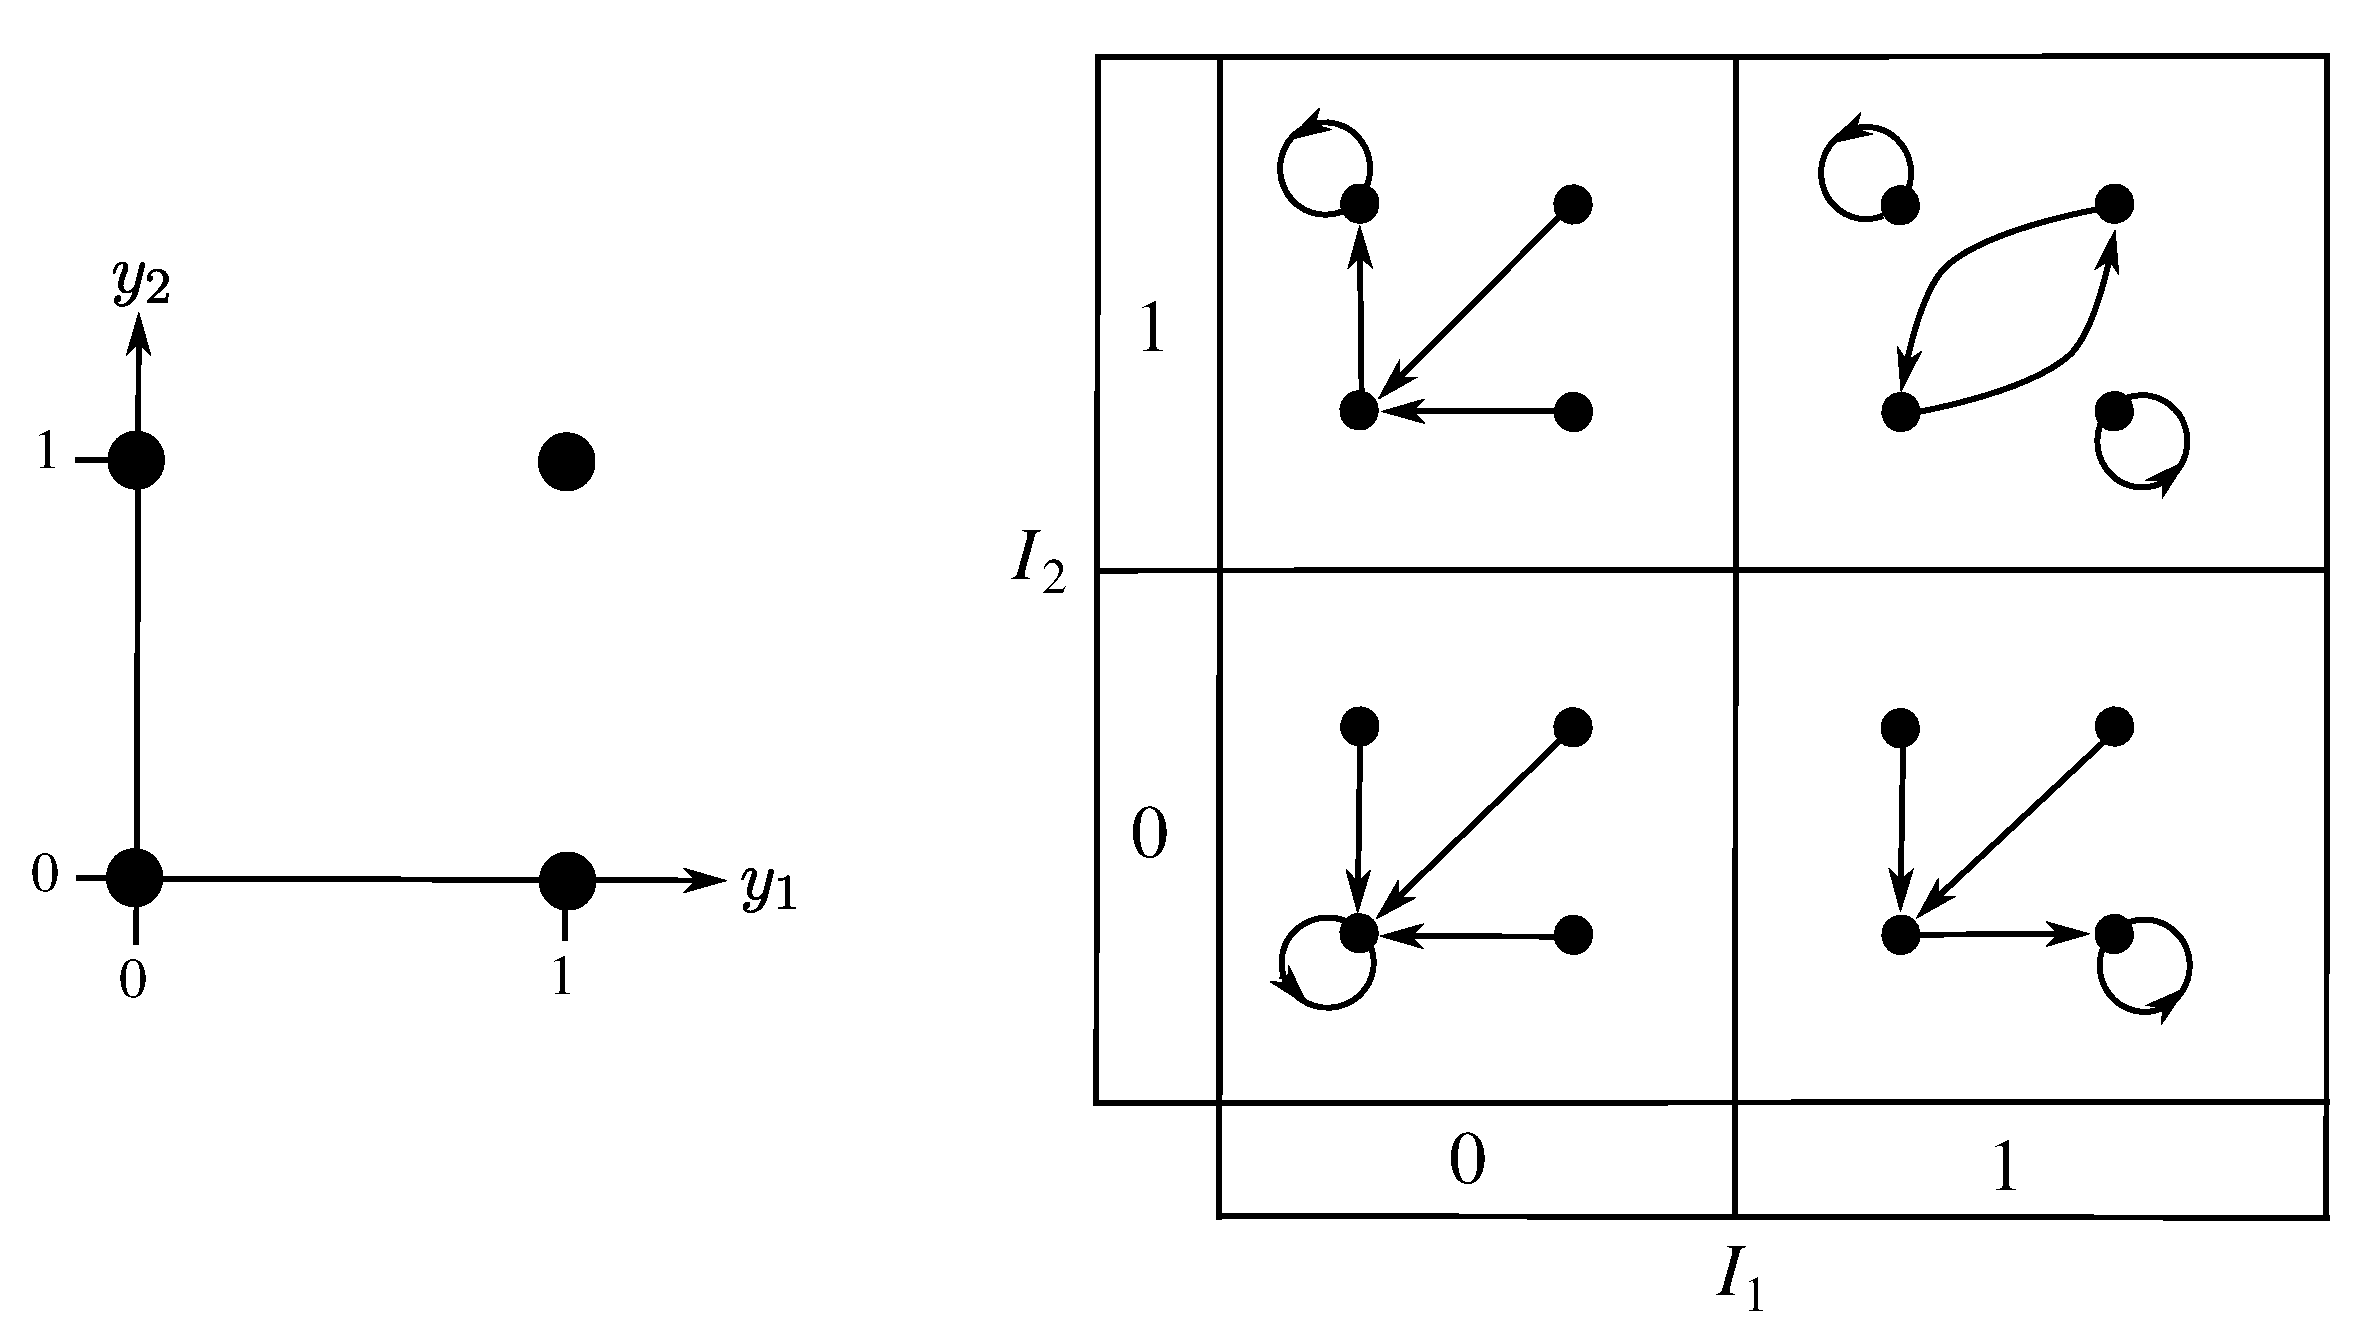
\includegraphics[scale=0.40]{./images/TwoNodeHopfield.pdf}
\caption{The dynamics for the Hopfield network with two discrete neurons. 
(Left) The state space for the neural network is the set of four vertices 
$\{0,1\}^2$.  (Right) The dynamics of the neural network is represented with 
digraphs on the state space for the four chosen input values for $(I_1,I_2)^T$. 
This is like a phase portrait for the discrete dynamical system.}
\label{F:TwoNodeHopfield}  
\end{figure}

   If both inputs are $0$ then the neural network goes to the state $(0,0)^T$ 
in one time step.  This state corresponds to the neural network recognizing 
that neither object is present.  If the input for the first object is $1$ and 
for the second object is $0$ then the neural network goes to the state $(1,0)$
in at most two time steps and once it is there it stays there, so long as the
inputs do not change.  This state corresponds to the neural network recognizing
that object 1 is present and object 2 is absent.  If the input for the first 
object is $0$ and for the second object is $1$ then the neural network goes to 
the state $(1,0)$ in at most two time steps and once it is there it 
stays there, so long as the inputs do not change.  This state corresponds to 
the neural network recognizing that object 2 is present and object 1 is absent.
In these three cases the neural network has a globally attracting fixed point
and it is the fixed point we want for the input.

   If both inputs are $1$ then the long term behavior depends on the state
that it is in during the present moment.  If it begins in a state that 
corresponds to recognizing the presence of one object and the absence of the 
other object then it will stay in that state for all time despite the fact that 
both objects are present\footnote{This resembles priming in perceptual 
psychology}.  If the network does not begin in a state that corresponds to 
recognizing the presence of one object and the absence of the other object then 
it will never go to such a state.  It will simply oscillate between the states 
$(0,0)^T$ and $(1,1)^T$\footnote{This resembles being in a confused mental 
state.}. 

   This neural network can recognize the absence of both objects and it can
recognize the presence of an object if the other object is absent.  If both
objects are present then it will only recognize an object if it is already in 
the state that corresponds to recognizing that object.  Otherwise it will
oscillate between the states $(0,0)^T$ and $(1,1)^2$.

  Hopfield's potential function is:
\begin{eqnarray*}
V
\begin{pmatrix}
y_1 \\  y_2
\end{pmatrix}
 &=& -\,\displaystyle{\frac{1}{2}} \left(
  \begin{matrix}\begin{pmatrix}y_1 & y_2\end{pmatrix}\\\mbox{}\end{matrix}
  \begin{pmatrix} 0 & -2 \\ -2 & 0 \end{pmatrix} 
  \begin{pmatrix} y_1 \\ y_2 \end{pmatrix} \right) 
-
\begin{pmatrix}
I_1 \\ I_2 
\end{pmatrix}
\bullet
\begin{pmatrix}
y_1 \\ y_2 
\end{pmatrix} \\
~ &=& 
  \begin{matrix}\begin{pmatrix}y_1 & y_2\end{pmatrix}\\\mbox{}\end{matrix}
  \begin{pmatrix} 0 & 1 \\ 1 & 0 \end{pmatrix} 
  \begin{pmatrix} y_1 \\ y_2 \end{pmatrix} 
-
\begin{pmatrix}
I_1 \\ I_2 
\end{pmatrix}
\bullet
\begin{pmatrix}
y_1 \\ y_2 
\end{pmatrix} = 2 y_1 y_2 - I_1 y_1 - I_2 y_2
\end{eqnarray*}
The values of the potential function on the state space $\{0,1\}^2$ can be
easily computed.  They are shown in Fig. \ref{F:discHoppot}.  The directed 
edges point to the subsequent state.  As can be seen from the figure the 
potential function never increases with time.  And each fixed point is a 
minimum of the potential although they are not always the only minima.

\begin{figure}[ht]
\centering
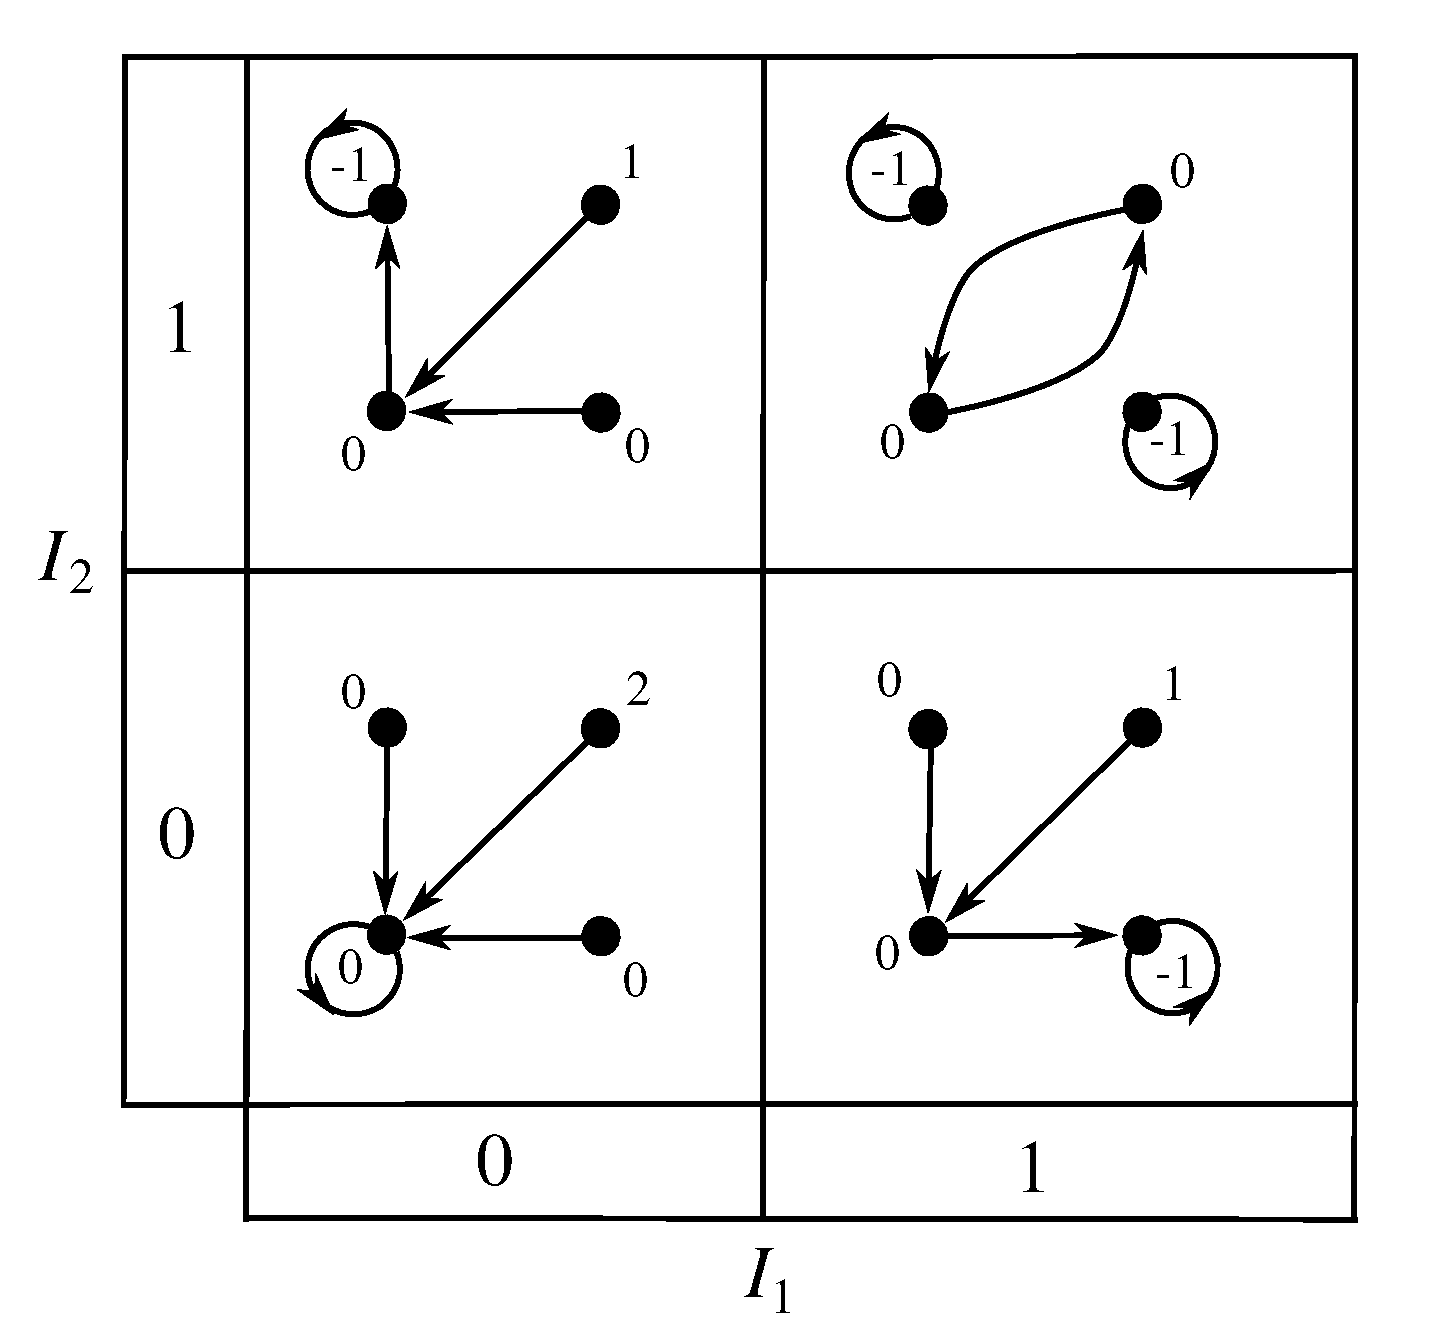
\includegraphics[scale=0.40]{./images/discHoppot.pdf}
\caption{The potential function $V(y_1, y_2)$ for the four chosen input 
values for $(I_1,I_2)^T$ along with the phase portrait.  The value of the 
potential function is labeled next to each state.}
\label{F:discHoppot}  
\end{figure}
  
\subsubsection{Asynchronous update}

   With asynchronous update we only update one neuron at a time in the neural 
network.  The two types of asynchronous update, sequential and stochastic,
only differ in how we select the neurons to update.  Let $n \in \{1,2\}$ stand 
for which neuron has been selected to be updated.  We still apply rules 
\eqref{E:hopinput} and \eqref{E:hopIO} to obtain a function that gives us the 
state $(y_1(t+1), y_2(t+1))^T$ in terms of the state $(y_1(t), y_2(t))^T$ but 
for rule \eqref{E:hopinput} we only use the component $x_n(t)$ in the vector 
$(x_1(t), x_2(t))^T$.  We then apply rule \eqref{E:hopIO} to $x_n(t)$ to get 
$y_n(t+1)$.

   The update function for neuron $1$ is:
\begin{equation}\label{E:hopexam1}
F_1
\left(
\begin{pmatrix}
y_1(t) \\ y_2(t)
\end{pmatrix},
\begin{pmatrix}
I_1 \\ I_2
\end{pmatrix}
\right)
=
\left\{
\begin{array}{ll}
(0,y_2(t))^T & \mbox{if} \quad y_2(t) \geq I_1/2 \\
(1,y_2(t))^T & \mbox{if} \quad y_2(t) < I_1/2 
\end{array}\right.
\end{equation}

   The update function for neuron $2$ is:
\begin{equation}\label{E:hopexam1}
F_2
\left(
\begin{pmatrix}
y_1(t) \\ y_2(t)
\end{pmatrix},
\begin{pmatrix}
I_1 \\ I_2
\end{pmatrix}
\right)
=
\left\{
\begin{array}{ll}
(y_1(t),0)^T & \mbox{if} \quad y_1(t) \geq I_2/2 \\
(y_1(t),1)^T & \mbox{if} \quad y_1(t) < I_2/2 
\end{array}\right.
\end{equation}
We can compute sequential update and stochastic update by composing these two 
functions on the state space $\{0,1\}^2$.  The digraphs for these two functions 
are shown in Fig.  \ref{F:TwoNodeHopfieldSingle}.  We can obtain the digraph 
for $F_1$ by using the formula for $F_1$ or by redirecting the arrows in Fig. 
\ref{F:discHoppot} so that only $y_1$ changes.  This is shown on the left in
Fig. \ref{F:TwoNodeHopfieldSingle}.  Similarly we can obtain the digraph for 
$F_2$ from the formula or by redirecting the arrows in Fig. \ref{F:discHoppot} 
so that only $y_2$ changes.  This is shown on the right in Fig.  
\ref{F:TwoNodeHopfieldSingle}.

\begin{figure}[ht]
\centering
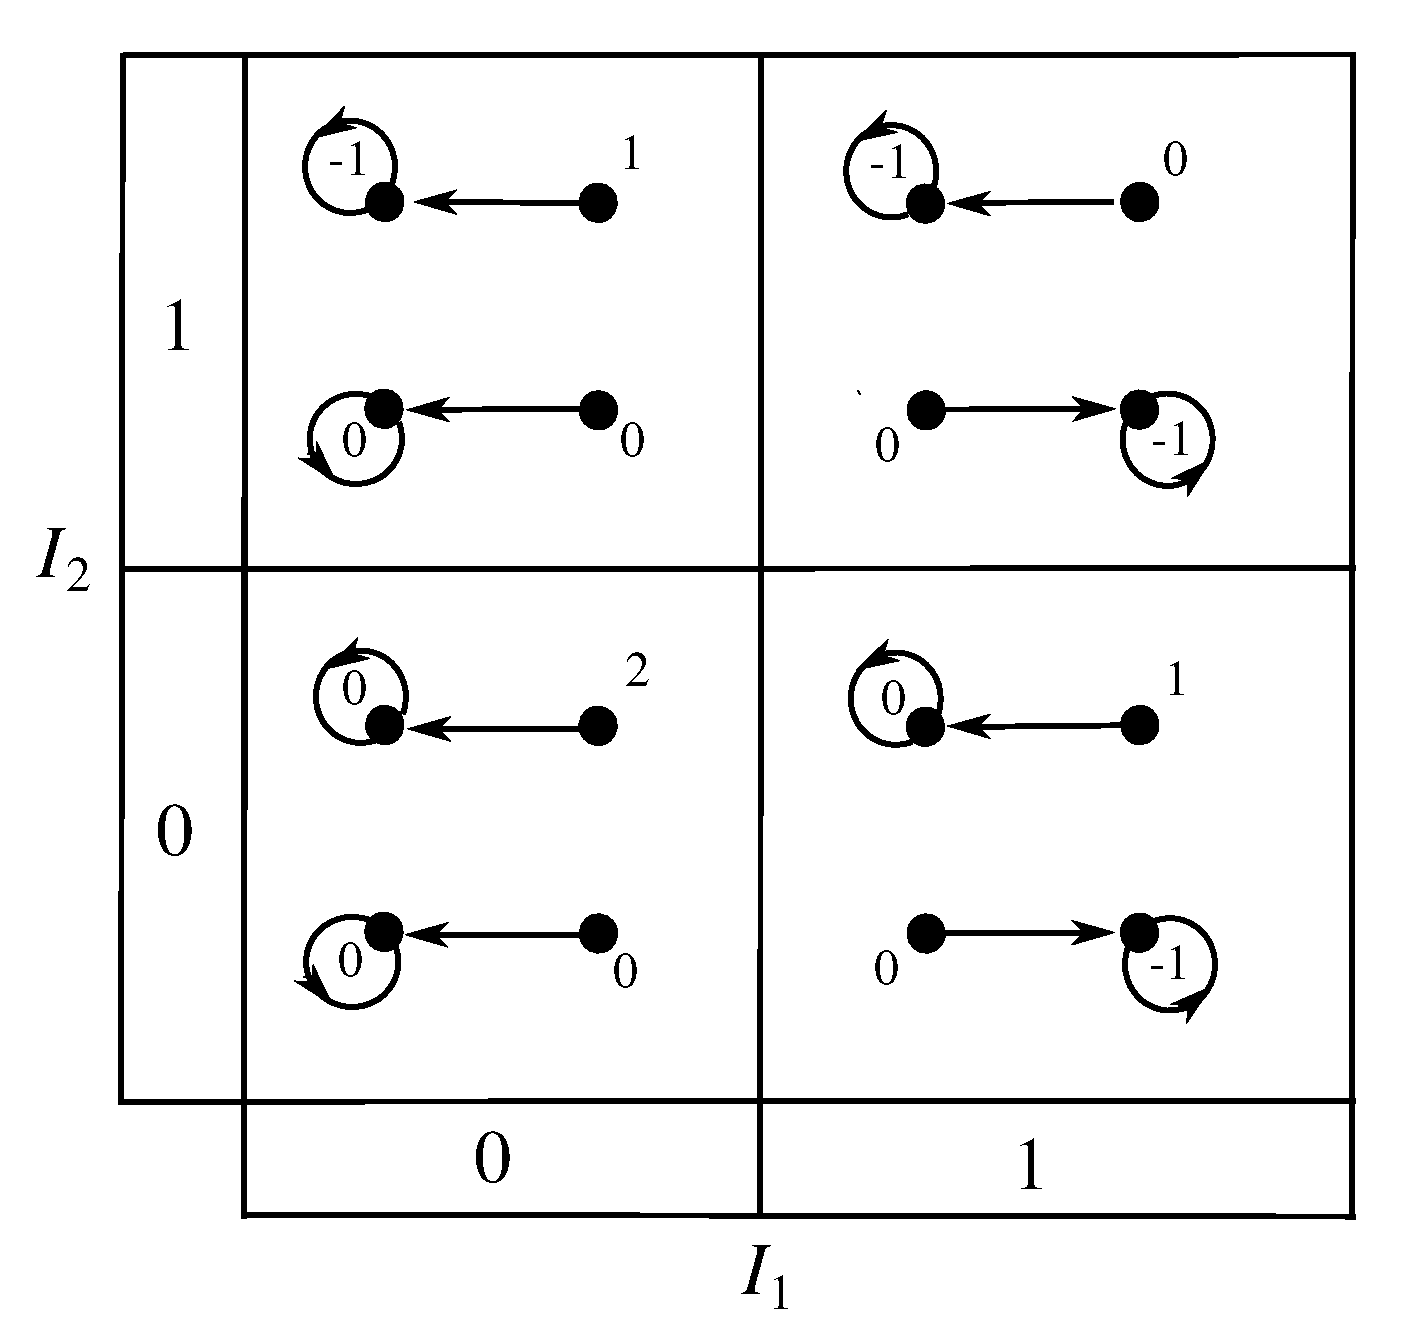
\includegraphics[scale=0.342]{./images/TwoNodeHopfieldUpdate1.pdf}
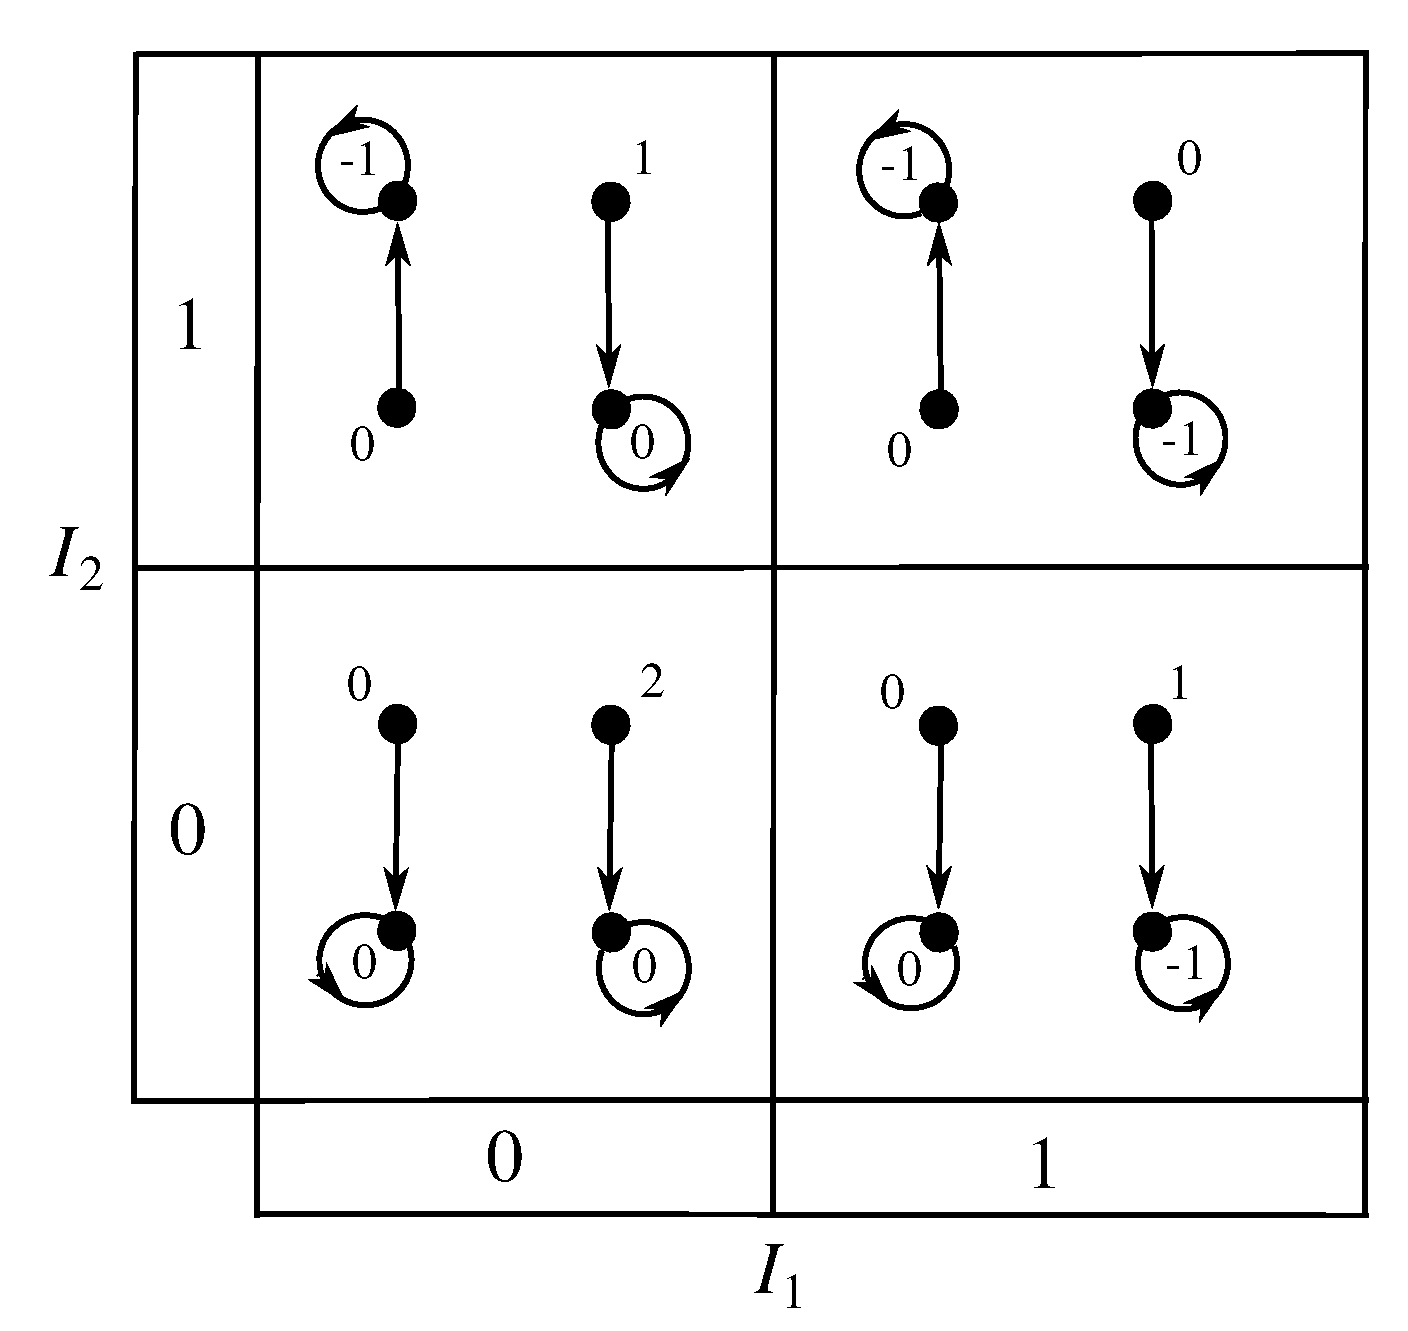
\includegraphics[scale=0.342]{./images/TwoNodeHopfieldUpdate2.pdf}
\caption{Digraphs for the functions on the state space $\{0,1\}^2$ when only 
one neuron is updated at time.  The value of the potential function 
$V(y_1,y_2)$ is labeled next to each state.  (Left) The digraphs for the 
function $F_1$, only neuron 1 can change its activation.  (Right) The digraphs 
for the function $F_2$, only neuron 2 can change its activation.  For each 
input vector there are two attracting fixed points.  Which fixed point the 
system ends up in depends on the initial state.  If the input vector is not 
$(1,1)^T$ the fixed point may or may not match the input.  If the input vector 
is $(1,1)^T$ then the fixed points do not match the input.}
\label{F:TwoNodeHopfieldSingle}
\end{figure}

  In addition Fig. \ref{F:TwoNodeHopfieldSingle} shows that $F_1$ and $F_2$ 
never increase the value of the potential function $V(y_1,y_2)$.  So composing 
them never increases the value of $V(y_1,y_2)$.  In this respect asynchronous
update is like synchronous update.

\subsubsection{Sequential update} 

  With just two nodes there are just two possible sequences for the nodes.
We either start with neuron $1$ and go to neuron $2$ or we start with neuron 
$2$ and go to neuron $1$.  
\begin{eqnarray*}
\begin{pmatrix}
y_1(t+1) \\ y_2(t+1)
\end{pmatrix}
= 
F_{12}
\left(
\begin{pmatrix}
y_1(t) \\ y_2(t)
\end{pmatrix},
\begin{pmatrix}
I_1 \\ I_2
\end{pmatrix}
\right)
=
F_1
\left(
F_2
\left(
\begin{pmatrix}
y_1(t) \\ y_2(t)
\end{pmatrix},
\begin{pmatrix}
I_1 \\ I_2
\end{pmatrix}
\right),
\begin{pmatrix}
I_1 \\ I_2
\end{pmatrix}
 \right) \\
\begin{pmatrix}
y_1(t+1) \\ y_2(t+1)
\end{pmatrix}
= 
F_{21}
\left(
\begin{pmatrix}
y_1(t) \\ y_2(t)
\end{pmatrix},
\begin{pmatrix}
I_1 \\ I_2
\end{pmatrix}
\right)
=
F_2
\left(
F_1
\left(
\begin{pmatrix}
y_1(t) \\ y_2(t)
\end{pmatrix},
\begin{pmatrix}
I_1 \\ I_2
\end{pmatrix}
\right),
\begin{pmatrix}
I_1 \\ I_2
\end{pmatrix}
 \right)
\end{eqnarray*}
The digraphs for these two functions are shown in Fig.  
\ref{F:TwoNodeHopfieldSequence}.  We can obtain the digraph for $F_{12}$ by
seeing where states go in the digraph for $F_2$ in Fig. 
\ref{F:TwoNodeHopfieldSingle} and then where those states go in the digraph for
$F_1$.  To obtain the digraph for $F_{21}$ we look at where states go in the
digraph for $F_1$ and then where those states go in the digraph for $F_2$.

\begin{figure}[ht]
\centering
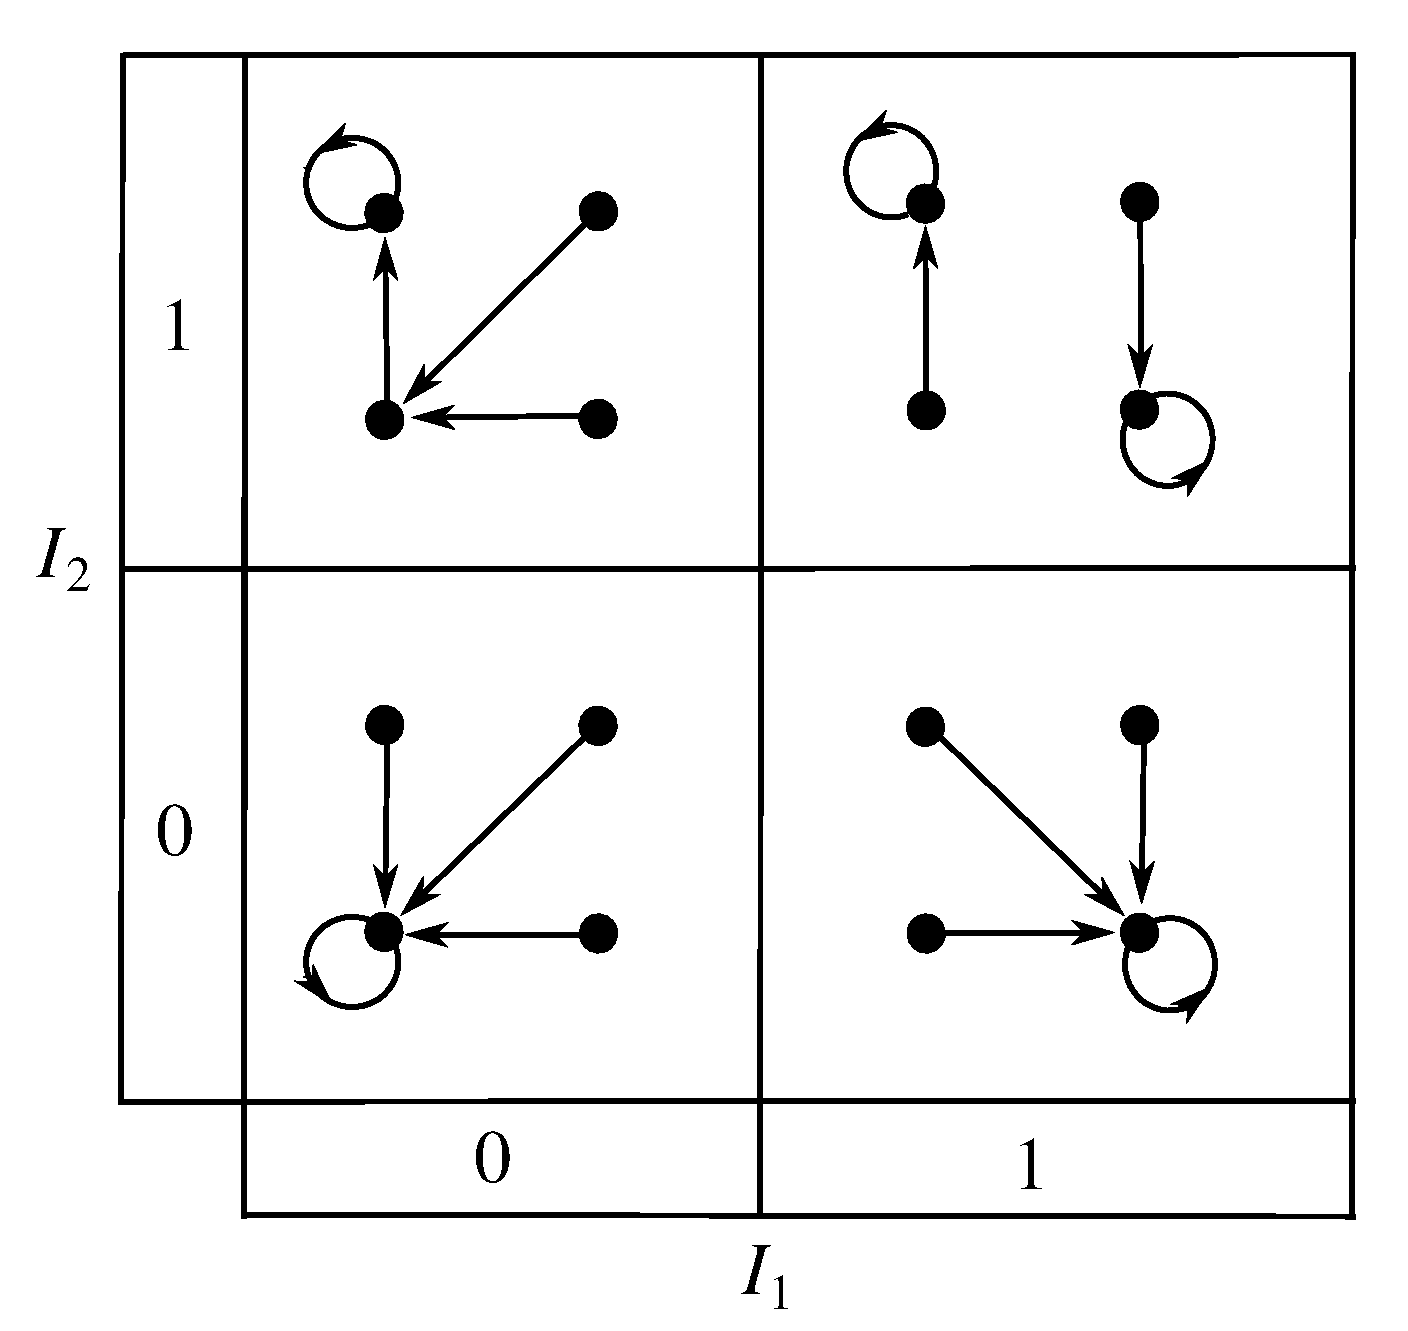
\includegraphics[scale=0.342]{./images/TwoNodeHopfieldUpdate12.pdf}
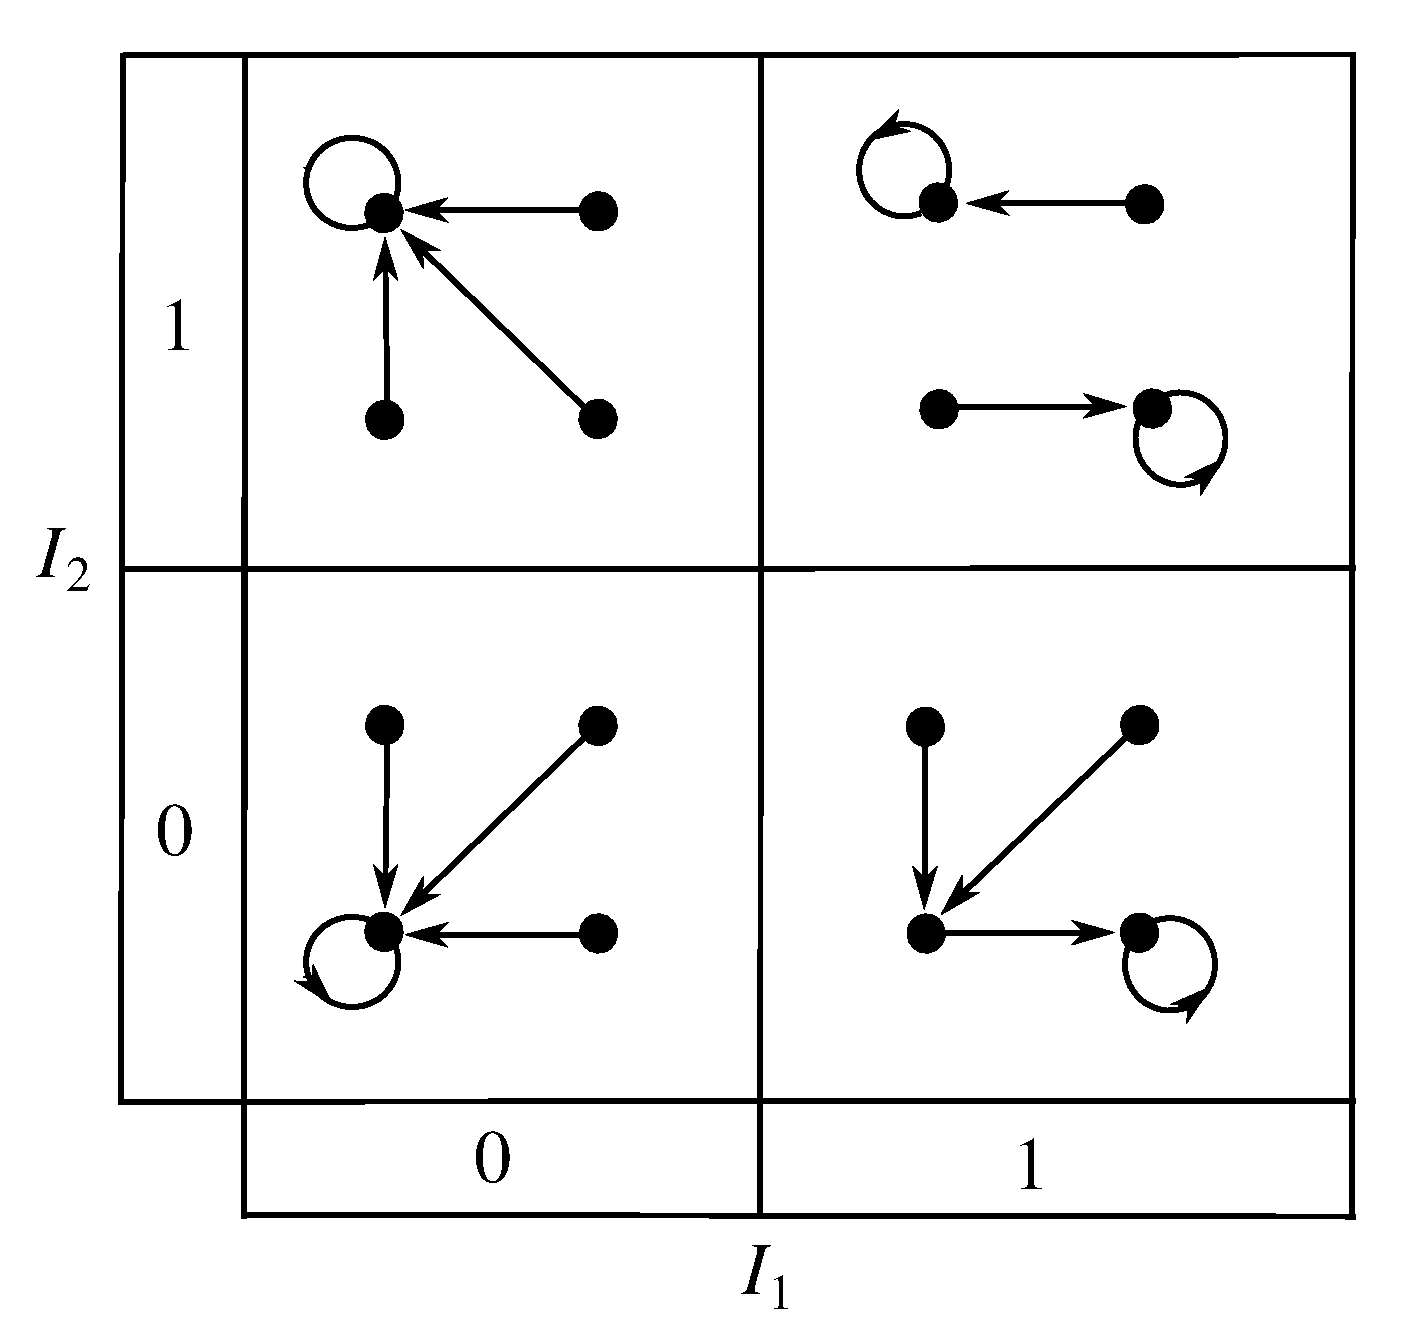
\includegraphics[scale=0.342]{./images/TwoNodeHopfieldUpdate21.pdf}
\caption{Digraphs for the dynamical systems obtained by sequential update. 
(Left) The dynamical systems obtained by iterating $F_{12}$ for each input.  
(Right) The dynamical systems obtained by iterating $F_{21}$ for each input.  
If the input vector is not $(1,1)^T$ then the system has a globally attracting 
fixed point and it matches the input vector.  If the input vector is $(1,1)^T$ 
then the fixed points are $(1,0)$ and $(0,1)$.  Which fixed point the system 
ends up in depends on the initial state.}
\label{F:TwoNodeHopfieldSequence}  
\end{figure}

   As with synchronous update the dynamical systems obtained by iterating 
$F_{12}$ or $F_{21}$ go to the fixed point we want for the input so long as 
the input vector is not $(1,1)^T$.  If the input vector is $(1,1)^T$ then the 
dynamical systems go to one of the fixed points $(1,0)^T$ or $(0,1)^T$.  Unlike
with synchronous update neither $F_{12}$ nor $F_{21}$ produce oscillations in 
the state space.  If both inputs are $1$ the network will recognize the 
presence of just one of the objects.  Which object it detects depends on the 
initial state and the order in which we update the neurons.

\subsubsection{Stochastic update} 

   In stochastic update we select which neuron to update randomly.  In this 
section we will use a uniform probability function to make the selection.  
So the probability for each neuron being selected is $1/2$.  The functions 
$F_1$ and $F_2$ are the update functions for neuron 1 and neuron 2 
respectively.  To analyze stochastic update it is useful to combine the 
digraphs for $F_1$ and $F_2$ in Fig. \ref{F:TwoNodeHopfieldSingle} into a
single digraph.  This union of digraphs is shown in Fig. 
\ref{F:TwoNodeHopfieldStochastic}.  
   
   The functions $F_1$ and $F_2$ have the same domain and range which is the
set of vertices of a square.  So each of the digraphs for $F_1$ and $F_2$ have 
the same set of vertices which is $\{0,1\}^2$.  The digraphs for $F_1$ and 
$F_2$ only differ in having some of their directed edges be different.   

   Because the digraphs stand for functions each vertex has exactly one edge 
directed away from it.  If $F_1$ and $F_2$ have the same value at a vertex then
their digraphs have the same edge directed away from that vertex.  In the 
union of the digraphs for $F_1$ and $F_2$ this vertex has just that one edge
directed away from it.  If $F_1$ and $F_2$ do not have the same value at a 
vertex then their digraphs have different edges directed away from that vertex.
In the union of the digraphs for $F_1$ and $F_2$ this vertex has these two 
edges directed away from it.  This can be checked in Figs. 
\ref{F:TwoNodeHopfieldSingle} and \ref{F:TwoNodeHopfieldStochastic}.  

\begin{figure}[ht]
\centering
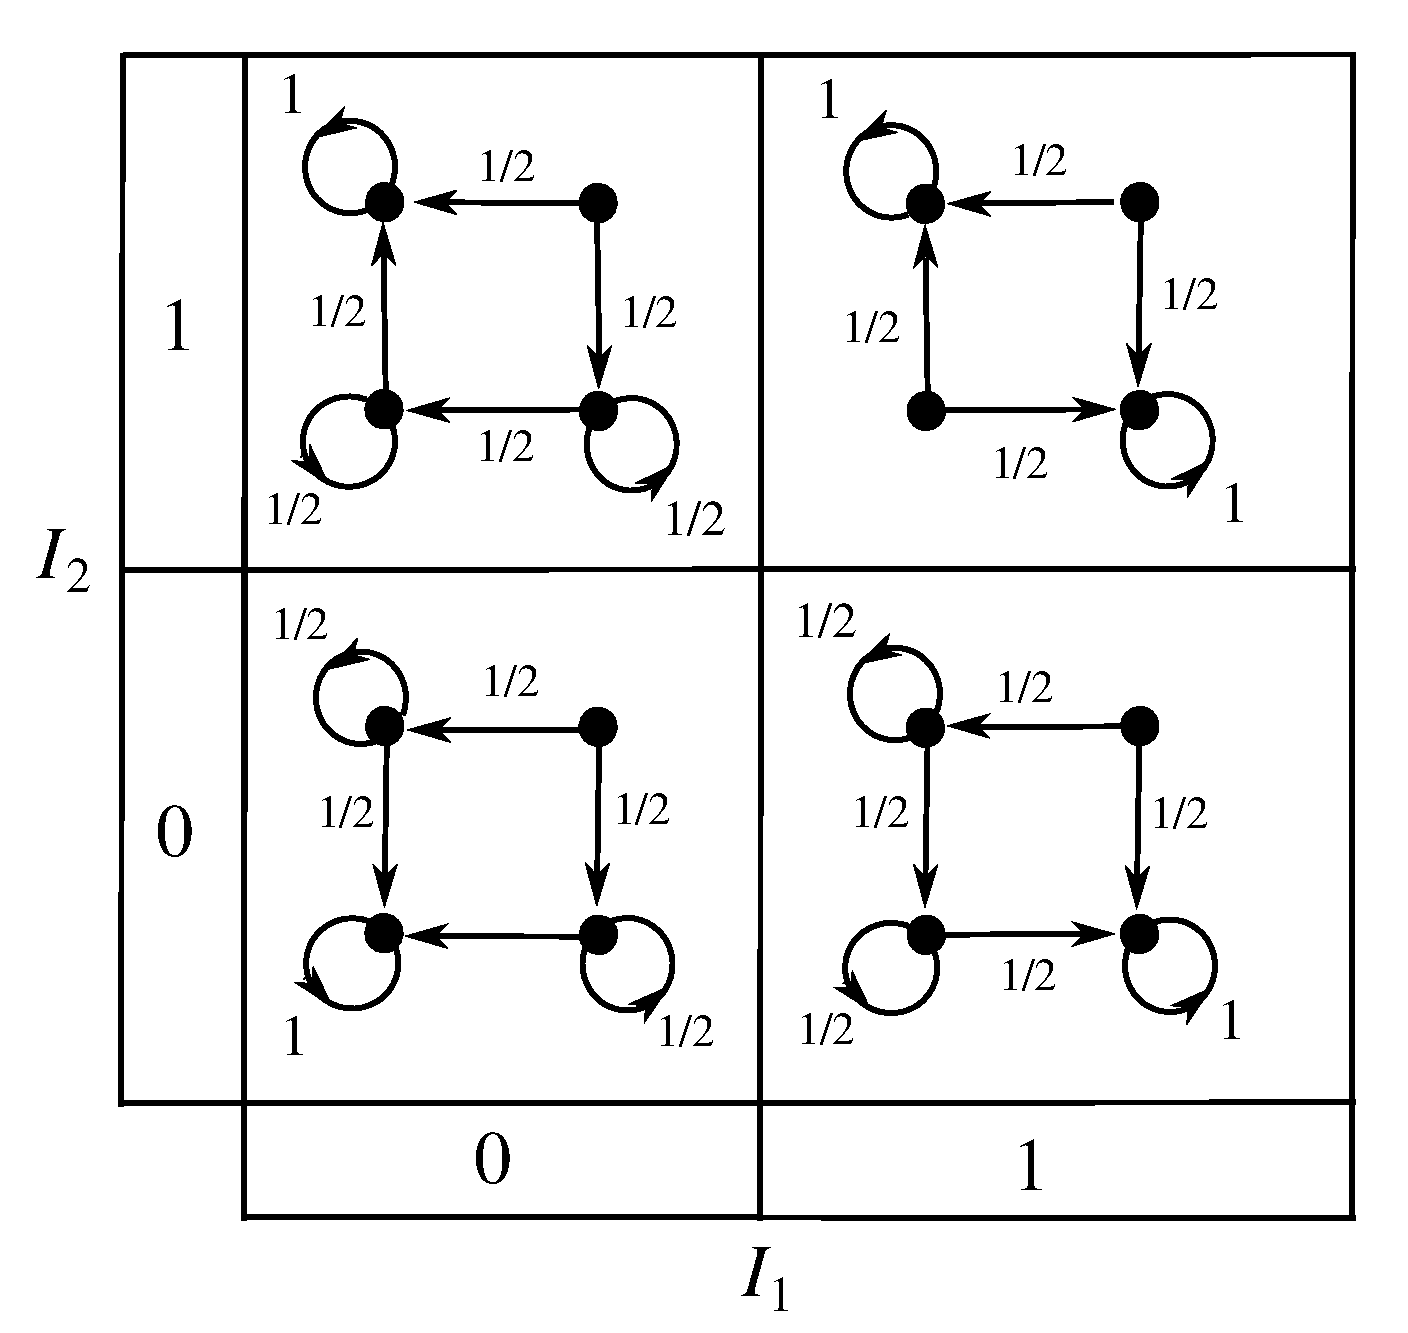
\includegraphics[scale=0.45]{./images/TwoNodeHopfieldMarkov.pdf}
\caption{Stochastic update where the neuron to update is randomly selected with 
a probability of $1/2$ is represented with a transition diagram.  The states
are indicated by the dots and the arrows between the dots indicate the possible 
transitions between states.  Each arrow is labeled with the probability that the
transition will occur.  If the input vector is not $(1,1)^T$ then the system 
eventually reaches the state that matches its input.  If the input vector is 
$(1,1)^T$ and the system starts out in $(1,0)^T$ or $(1,0)^T$ then it will
stay in its starting state, otherwise it eventually reaches either $(1,0)^T$ or 
$(1,0)^T$ with probability of $1/2$, and stays there.} 
\label{F:TwoNodeHopfieldStochastic}  
\end{figure}

   When $F_1$ and $F_2$ have the same value at a vertex then the probability 
that the network will transition to that state is $1$.  In the union of the
digraphs for $F_1$ and $F_2$ we label the edge directed away from the vertex
with a $1$ to indicate that the probability for that transition to occur is 
$1$.  

   When $F_1$ and $F_2$ have different values at a vertex then there are two 
states the network can transition to.  Since the probability for a neuron to be
selected is $1/2$ the probability for each of the transitions is $1/2$.  In the 
union of the digraphs for $F_1$ and $F_2$ we label the two edges directed away 
from the vertex with $1/2$ to indicate that the probability for that transition 
to occur is $1/2$.

   These digraphs with their edges labeled with probabilities are known as 
transition digraphs, transition graphs, and as transition diagrams for a Markov
process.  As we said at the beginning of this section a Markov process is a 
stochastic process for which future states only depend on the present state.  A 
Hopfield network with stochastic update is a Markov process.  The future states 
of a Hopfield network only depend on the present state and how the neurons are 
randomly selected to be updated.  Fig. \ref{F:TwoNodeHopfieldStochastic} shows 
the transition diagram for the Markov process in this example Hopfield network.

   There is a well developed theory for Markov processes but the Markov
processes in this example Hopfield network are particularly simple cases of 
Markov processes.  So we will not need to use very much from the theory of 
Markov processes.

   If the only edge directed from a vertex is also directed towards itself then
the vertex is called an absorbing state of the Markov process.  The presence of
absorbing states simplifies the analysis of a Markov process.  Once a Markov 
process reaches an absorbing state it does not leave.  

   It can be seen from the transition diagram that when the input vector is not 
$(1,1)^T$ there is exactly one absorbing state in the neural network's state 
space.  Moreover each of these absorbing states matches the input vector.  When 
the input vector is $(1,1)^T$ there are two absorbing states, $(1,0)^T$ and 
$(0,1)^T$.

   It can be seen from the transition diagram that the neural network state 
$(1,1)^T$ has no edges directed towards it.  This means that the neural 
network can not remain in the state $(1,1)^T$ and once it leaves it does not 
return.

  It can also be seen from the transition diagram that, except for the state
$(1,1)^T$, each of the non-absorbing states can transition to themselves.  For 
each of these non-absorbing states there are no other directed paths in the 
digraph that begin and end with them.  Once the Hopfield network leaves one of these states it does not return.

   For each of the non-absorbing states that can transition to themselves the
probability that it will transition to itself in one time step is $1/2$.  The
probability that it will transition to itself in two time steps is $(1/2) \cdot
(1/2) = 1/4$.  The probability that it will transition to itself in $k$ time 
steps is $1/2^k$.  This probability goes to $0$ as $k$ is increased without
bound.  So as we keep performing stochastic update the probability that it
will transition away from itself goes to $1$.  We say it is almost certain that
it will transition away from itself.  This is like flipping a coin until it
stops landing heads.  It is almost certain that sooner or later you will stop 
flipping the coin.

   So eventually the Hopfield networks will transition away from each 
non-absorbing state without returning.  Therefore they eventually end up in an 
absorbing state.  When the input vector is not $(1,1)^T$ there is a unique 
absorbing state and it matches the input vector.  When the input vector is 
$(1,1)^T$ the absorbing states are $(1,0)^T$ and $(0,1)^T$.  If the neural 
network does not begin in one of these absorbing states then which one it ends 
up in is random.  The probability of ending up in one of these two absorbing 
states is $1/2$.

  With stochastic update the Hopfield network can recognize the absence of
both objects and it can recognize the presence of one object when the other
object is not present.  If both objects are present it random enters one of the
states for the presence of a single object.

\subsubsection{Summary}

   In summary the long term behavior for the synchronous, sequential, and 
stochastic update methods is the same when the input vector is not $(1,1)^T$.  
The system goes to the state that matches the input and stays there.  When the 
input vector is $(1,1)^T$ the points $(0,0)^T$ and $(1,1)^T$ form a 2-cycle of 
the dynamical system for synchronous update but for sequential and stochastic 
update the network eventually ends up in either the state $(1,0)^T$ or the 
state $(0,1)^T$.

\section{Boltzmann Machines}

This is a variant on a Hopfield network that has a probabilistic element. Neurons are updated by taking a sigmoid rule on weighted inputs to determine a probability of firing.  Such a network can be thought of as something like a Spin glass or Ising network, where the nodes are like magnets and their overall behavior is governed by weights and they will tend to settle into a pattern, just like Hopfield, but in more stochastic way.  Weights are intuitively like correlations, where positive weights correspond to nodes that are typically both on and negative weights corresponds to nodes that are anti-correlated so that one is on when the other is off.

Learning occurs by exposing the network to a training pattern, running the network, observing the difference, and updating the weights in a way that will make the network tend to settle into the training pattern state.

Then a restricted Boltmzann machine is a trick where to make things simpler, we separate visible and hidden nodes, and the learning just happens on the weight between the visible and hidden layers (which are shared).  So the hidden nodes pick up on the statistics of the visible layer.

They also use an energy landscape, They tend to settle into low-energy states, so that we can draw on thermodynamics analogies. There are some differences in interpretation though.

But the whole thing basically acts like a stochastic version of a Hopfield network, a markov process that tends towards a few states that correspond to the fixed points of a Hopfield net.

Summary of room schema.

An actual use is to reccomend movies. Put in a person's set of preferred movies. Now put in a subset. The network figures out the rest. But feed-forward models can do this, and probably better, so they fell out in engineering.

% Makes sure figure attributions are listed in table of contents
\phantomsection 
\addcontentsline{toc}{chapter}{Figure Attributions} 
\listoffigures

% Makes sure references are listed in table of contents
\phantomsection 
\addcontentsline{toc}{chapter}{References} 
\bibliography{NeuralNetworksCogsci}{}
\bibliographystyle{plain}

\end{document}
